% Page settings
\documentclass[notitlepage,12pt]{article}
\usepackage{fancyvrb, verbatim, listings}                                  % Various for inserting/hosting code
\usepackage{setspace}                                                      % Space between lines (customisable)
\usepackage[margin=2.54cm]{geometry}                                       % Set margins (standard is 2.54cm)
\usepackage[UKenglish,cleanlook]{isodate}                                  % Set default date and date display
\usepackage{fancyhdr} \pagestyle{fancy}                                    % Line the top of the page
\usepackage[activate={true,nocompatibility},final,tracking=true,kerning=true,spacing=true,factor=1100,stretch=10,shrink=10]{microtype}
\microtypecontext{spacing=nonfrench}                                       % Change font and minor spacings to look nicer
\setlength{\parskip}{0.5\baselineskip}                                     % Set default paragraph behaviour: skip a line
%\setlength{\parindent}{0pt}                                                % Set default paragraph behaviour: no indent
%% Packages to use:
% Tables + figures
\usepackage{graphicx}                                                      % control over the import of graphics
\usepackage[table,dvipsnames]{xcolor}                                      % Define tables (with colour control)
\usepackage{float}                                                         % Control over graphics + tables float
\usepackage[justify]{ragged2e}                                             % control over text alignment
\usepackage{booktabs}                                                      % caption graphics + tables (with name in bold)
\usepackage[labelfont=bf]{caption} 
\usepackage{subcaption}
\usepackage[shortlabels]{enumitem}                                         % Customisable lists
% caption graphics + tables (with name in bold)
\usepackage{tikz}
\usetikzlibrary{shapes,decorations,decorations.pathreplacing,arrows,calc,arrows.meta,fit,positioning}
\tikzset{
    auto,node distance =1 cm and 1 cm,semithick,
    state/.style ={ellipse, draw, minimum width = 0.7 cm},
    point/.style = {circle, draw, inner sep=0.04cm,fill,node contents={}},
    bidirected/.style={Latex-Latex,dashed},
    el/.style = {inner sep=2pt, align=left, sloped}
}
%\usepackage{pgfplots} \pgfplotsset{compat=1.16}                            % Automatic graphing, read https://www.overleaf.com/learn/latex/pgfplots_package for examples
% Maths + numbers
\usepackage{mathtools}                                                     % Various maths functions
\usepackage{amssymb}                                                       % Various maths functions
\usepackage{amsmath}                                                       % Various maths functions
\usepackage{dsfont}                                                        % Various maths functions
\usepackage{centernot}                                                     % center \not usage
\usepackage{siunitx} \sisetup{round-mode=places, round-precision=3}        % Formalise use of units and numbers among text
\usepackage{amsthm}                                                        % NEvrionemtn for theorems.
\newtheorem{theorem}{Theorem}                                              % Define theorem environment.
\newtheorem{assumption}{Assumption}                                        % Define assumptions environment ahead of theorems.
\newtheorem{definition}{Definition}                                        % Define definitions environment ahead of theorems.
\DeclareMathOperator{\eps}{\varepsilon}                                    % epsilon short hand shortcut
\DeclareMathOperator{\st}{\text{ s.t. }}                                   % "such that" short hand shortcut
\DeclareMathOperator{\then}{\text{ then }}                                 % "then" in equation shortcut
\DeclareMathOperator{\ifeq}{\text{ if }}                                   % "if" in equation shortcut
\DeclareMathOperator{\oreq}{\text{ or }}                                   % "or" in equation shortcut
\DeclareMathOperator{\andeq}{\text{ and }}                                 % "and" in equation shortcut
\DeclareMathOperator{\all}{,\; \text{ for }}                                    % all (with spacing) in equation shortcut
\DeclareMathOperator{\N}{\mathbb{N}}                                       % N, natural number, shortcut
\DeclareMathOperator{\R}{\mathbb{R}}                                       % R, real number, shortcut
\DeclareMathOperator{\Ll}{\mathcal{L}}                                     % L, Lagrangian, shortcut
\renewcommand{\vec}[1]{\boldsymbol{\mathit{#1}}}                           % vector notation shortcut
\newcommand{\mat}[1]{\boldsymbol{\mathit{#1}}}                             % matrix notation shortcut
\DeclarePairedDelimiter\abs{\lvert}{\rvert}                                % absolute value notation shortcut
\DeclarePairedDelimiter\norm{\lVert}{\rVert}                               % norm notation shortcut
\newcommand{\Prob}[1]{\Pr\left( #1 \right)}                         % SHortcut for probability notation
\newcommand{\Probgiven}[2]{\Pr\left( #1 \, \middle\vert \, #2 \right)} % SHortcut for probability notation, given
\newcommand{\E}[2][]{\mathbb{E}_{#1} \left[ #2 \right]}                    % Expectation (with optional subscript) shortcut
\newcommand{\Egiven}[3][]{\mathbb{E}_{#1} \left[ #2 \, \middle\vert \, #3 \right]} % Expectation given (with optional subscript) shortcut
\newcommand{\Var}[2][]{\text{Var}_{#1} \left( #2 \right)}                  % Variation (with optional subscript) shortcut
\newcommand{\Cov}[1]{\text{Cov} \left( #1 \right)}                         % Covariance (with optional subscript) shortcut
\newcommand{\median}[1]{\text{median} \left( #1 \right)}                   % Median (with optional subscript) shortcut
\newcommand{\indicator}[1]{\mathds{1}\left\{ #1 \right\}}                  % SHortcut for indicator function
\newcommand{\diff}[2][]{\frac{d#1}{d#2}}                                   % SHortcut for differential fraction as a function
\newcommand{\partialdiff}[2][]{\frac{\partial#1}{\partial#2}}              % SHortcut for partial differential fraction as a function
\newcommand{\converge}[1]{\xrightarrow{ #1 \to\infty}}                     % SHortcut for convergence arrow
\renewcommand{\hat}[1]{\widehat{#1}}                                       % Default estimator notation is widehat
\renewcommand{\bar}[1]{\overline{#1}}                                      % Make over bar look nicer
\renewcommand{\tilde}[1]{\widetilde{#1}}                                   % Make over tilde look better
\newcommand{\indep}{\, \raisebox{0.05em}{\rotatebox[origin=c]{90}{$\models$}} \,}% Statistical independence symbol.
\definecolor{ao(english)}{rgb}{0.0, 0.5, 0.0}                              % Define dark green colour 
% Citations
\usepackage{natbib} %[longnamesfirst]                                  % Citation package, see https://en.wikibooks.org/wiki/LaTeX/Bibliography_Management#Natbib
\usepackage[backref=page]{hyperref}                                        % Allow for links across the text, with colour options
\hypersetup{colorlinks=true, linkcolor=blue, citecolor=blue, filecolor=magenta, urlcolor=blue}
\def\sectionautorefname~#1\null{Section~#1\null}                           % Fix autoref for sections
\def\subsectionautorefname~#1\null{Subsection~#1\null}                     % Fix autoref for subsections
\def\subsubsectionautorefname~#1\null{Subsubsection~#1\null}               % Fix autoref for subsubsections
\def\equationautorefname~#1\null{Equation~(#1)\null}                       % Fix autoref for equations
% IMPORTANT: follow style guide here https://github.com/Wookai/paper-tips-and-tricks
\usepackage{epigraph}                                                      % Package for quoting from elsewhere.


%%%%%%%%%%%%%%%%%%%%%%%%%%%%%%%%%%%%%%%%
%% Title page
% Author
\author{Senan Hogan-Hennessy\thanks{
    % This work has been supported by research grants from the Centre for the Study of Inequality and Economics Department, Cornell University.
    For helpful comments I thank
    Neil Cholli,
    Luk\'a\u{s} Laff\'ers,
    Hyewon Kim,
    Yiqi Liu,
    Douglas Miller,
    Zhuan Pei
    Brenda Prallon,
    and
    Evan Riehl.
    Some results in this paper previously circulated in an unpublished version of the working paper ``The Direct and Indirect Effects of Genetics and Education.''
    % I thank seminar participants at Cornell University (2025) for helpful discussion.
    Any comments or suggestions may be sent to me at \href{mailto:seh325@cornell.edu}{\nolinkurl{seh325@cornell.edu}}.
    %, or raised as an issue on the Github project.
    } \\
    \vspace{0.1cm}
    Economics Department, Cornell University\footnote{
        Address: Uris Hall \#447, Economics Department, Cornell University NY 14853 USA.
    }
}
% Title
\title{Causal Mediation in Natural Experiments}
\date{This version: \today \\ \vspace{0.25cm}
    \textbf{\textit{Unfinished, please do not circulate.}}
    %\textbf{\textit{Work-in-Progress, please do not circulate.}}
    %\href{https://github.com/shoganhennessy/mr-education}{Newest version available here.}
    \vspace{-0.5cm}
}
\rhead{\today}
\lhead{Causal Mediation in Natural Experiments.}
% Begin
\begin{document}
\clearpage
\maketitle
\thispagestyle{empty}
% Abstract
\begin{abstract}
    \noindent
Natural experiments are a cornerstone of applied economics, providing settings for estimating causal effects with a compelling argument for treatment ignorability.
Economists are often interested in understanding the mechanisms through which causal treatment effects operate, and Causal Mediation (CM) methods aid this by estimating how much of the treatment effect operates through a proposed mediator.
The most popular CM approach relies on assumptions which are unrealistic in natural experiment settings: assuming the mediator is conditionally ignorable --- in addition to the ignorability argument for the initial treatment.
This paper shows that this approach leads to biased inference, solving for explicit bias terms when the mediator is not ignorable.
Using the case of a Roy model for a mediator, I show that individuals' selection based on expected gains and costs is inconsistent with mediator ignorability without implausible behavioural assumptions, and that bias terms are large in practice.
I show a control function approach, which overcomes these hurdles if monotonicity holds, using cost of mediator take-up as an instrument.
Simulations confirm that this method corrects for persistent bias in conventional CM estimates, and performs comparably to a selection-on-observables approach when the structural assumptions do not hold.
% I illustrate the approach by estimating the proportion of the causal effect of genes associated with education that operates via a direct genetic channel versus indirectly through extended schooling.
% Finally, I provide an implementation of this method in the \textit{R} package \textit{mediate-controlfun}, offering an accessible tool for robust mediation analysis in natural experiment settings.
This approach gives applied researchers a practical method to estimate CM effects when they can only establish a credible argument for randomisation of the initial treatment, as is common in natural experiments.

\vspace{0.5cm}
\noindent
\textbf{Keywords:}
Direct/indirect effects, quasi-experiment, selection, control function.

\vspace{0.1cm}
\noindent
\textbf{JEL Codes:}
D31, D91, I24, J24, Z00.

\end{abstract}

%%%%%%%%%%%%%%%%%%%%%%%%%%%%%%%%%%%%%%%%%
%% Starting the paper
\newpage
\setcounter{page}{1}
\doublespacing
% Introduction section
\noindent
%\section{Introduction}
%\label{sec:intro}
% \textbf{The introduction formula \url{https://blogs.ubc.ca/khead/research/research-advice/formula}.}
%\textbf{Hook:}
Economists use natural experiments to credibly answer social questions, when an experiment was infeasible.
For example, does access to health insurance causally improve health and well-being \citep{finkelstein2008oregon}?
Natural experiments are settings which answer these questions, but give little indication of how these effects came about.
Causal Mediation (CM) aims to estimate the mechanisms behind causal effects, by estimating how much of the treatment effect operates through a proposed mediator.
For example, do causal gains from access to health insurance come mostly from starting to utilise healthcare more often, or are there other direct effects?
This study of mechanisms behind causal effects broadens the economic understanding of social settings studied with natural experiments.
This paper shows that the conventional approach to estimating CM effects is inappropriate in a natural experiment setting, provides a theoretical framework for how bias operates, and develops an approach to correctly estimate CM effects under alternative assumptions.
These methods contrast the current practice in applied economics of providing suggestive evidence of mechanisms, which does not identify or quantify causal effects.

% Paragraph here: how do applied economists currently do it?
% Summarise my work with the Finkelstein+ data.

%\textbf{Question:}
This paper starts by considering conventional CM methods in a natural experiment setting.
Conventional CM methods rely on assuming the initial treatment, and the subsequent mediator, are both ignorable \citep{imai2010identification}.
In a natural experiment setting, however, this may not hold true; 
winners of the Oregon Health Insurance Experiment wait-list lottery randomly received access to health insurance, but then chose of their own free will how often to use healthcare.
Here, conventional CM estimates for the average direct and indirect effects will be contaminated by bias terms, from not accounting for selection-into-healthcare.
Indeed, it is unlikely conventional CM estimates in any natural experiment will lead to credible causal effects, unless researchers use another natural experiment to isolate random variation in the mediator (at the same time as using one for the initial treatment).

I consider an alternative approach to estimating CM effects, adjusting for unobserved selection-into-mediator via identifying the marginal treatment effect of the mediator.
This solves the identification problem with structural assumptions for selection-into-mediator --- mediator monotonicity and selection based on benefits --- and requires a valid cost instrument for mediator take-up.
While these assumptions are strong, they are plausible in many applied settings.
Mediator monotonicity aligns with conventional theories for selection-into-treatment, and is accepted widely in many applications using an instrumental variables research design.
Selection based on costs and benefits is central to economic theory, and is the dominant concern for judging empirical designs that identify causal effects.
Access to valid instrumental variation is a strong condition, though is important to avoid further modelling assumptions; the most compelling example is using variation in mediator take-up costs as an instrument.
This approach is not perfect in every setting: the structural assumptions are strong, and are tailored to selection-into-mediator concerns pertinent to economic applications.
Indeed, this approach provides no safe harbour for estimating CM effects if these structural assumptions do not hold true.

%Paragraph on the results of the Oregon experiment.

%\textbf{Antecedents:}
Assuming the mediator is quasi-randomly assigned conveniently ignores selection by assuming either (1) people na\"ively made decisions to take or refuse a mediator, or (2) a researcher controlled for everything relevant to this decision.
This assumption might be reasonable when studying single-celled organisms in a laboratory --- their ``decisions'' are simple and mechanical.
Social scientists, however, study humans who make complex choices based on costs, benefits, and preferences --- which are only partially observed by researchers, at best.
Assuming a mediator is ignorable in social science contexts is often unrealistic.
In practice, the main setting where mediator ignorability becomes credible is when researchers find another natural experiment affecting the mediator --- a rare occurrence given how difficult it is to find one source of random variation for a treatment, let alone another independent source for a mediator, at the same time.

The applied economics literature has been hesitant to use explicit CM methods, instead providing suggestive evidence for mechanisms,\footnote{
    See \cite{blackwell2024assumption} for an overview of this approach, from the empirical politics literature.
} sometimes accompanied by a practice of controlling for a proposed mediator.
Neither of these approaches have a causal interpretation.
A new strand of the econometric literature has developed estimators for explicit CM analyses under a variety of strategies.
These include overlapping quasi-experimental research designs \citep{deuchert2019direct,frolich2017direct}, functional form restrictions \citep{heckman2015econometric,heckman2013understanding}, partial identification \citep{flores2009identification}, or a hypothesis test of full mediation through observed channels \citep{kwon2024testing} --- see \cite{huber2019review} for an overview.\footnote{
    An alternative method to estimate CM effects is ensuring treatment and mediator ignorability holds by a running two randomised controlled trials for both treatment and mediator, at the same time.
    This set-up has been considered in the literature previously, in theory \citep{imai2013experimental} and in practice \citep{ludwig2011mechanism}.
}
The new literature has arisen in implicit acknowledgement that suggestive evidence of mechanisms, or a conventional approach to CM, can lead to biased inference and needs alternative methods for credible inference.

%\textbf{Value-added:}
I develop a framework showing exactly how selection bias contaminates CM estimates when mediator choices are driven by unobserved gains --- settings where none of the natural experiment research designs in the previously cited papers apply (i.e., the mediator is not ignorable).
This provides a rigorous warning to applied economists against uncritically applying conventional CM methods to investigate mechanisms in natural experiments --- as is common in the applied fields of epidemiology, psychology, and medicine.
Selection based on costs and benefits, as in the \cite{roy1951some} model, is at odds with assuming a mediator is randomly assigned in an observational setting, so I import methods grounded in labour economic theory to solve the identification problem.

Identifying CM effects via the marginal treatment effect of the mediator requires mediator take-up respond only positively to the initial treatment (monotonicity), which implies mediator selection follows a selection model.
Second, it assumes that mediator take-up is motivated by mediator benefits.
Last, it requires a valid instrument for mediator take-up, to avoid relying on parametric assumptions on unobserved selection.
This approach to identifying CM effects imports insights from the instrumental variables literature, connecting the influential \cite{imai2010identification} approach to CM with the economics literature on selection-into-treatment and marginal treatment effects \citep{vytlacil2002independence,heckman2004using,heckman2005structural,florens2008identification,kline2019heckits}.
%\footnote{
%    Indeed, this paper does not invent control function methods, instead noting their applicability in this setting.
%    See \cite{wooldridge2015control,imbens2007nonadditive} for general overviews of the approach.
%}
\cite{frolich2017direct} have previously explored identification of CM effects with a control function in the context of two instruments (one each for treatment and mediator) and a continuous mediator.
This paper considers the marginal treatment effect of a binary mediator, with a correspondingly different identification analysis and resulting estimation strategies.

%\textbf{Road-map:}
This paper proceeds as follows.
\autoref{sec:lottery} describes the dominant approach in economics for studying mechanisms behind treatment effects, illustrating with data from the Oregon Health Insurance Experiment.
% and surveys economic research.
\autoref{sec:mediation} introduces the formal framework for CM, and develops expressions for bias in CM estimates in natural experiments.
\autoref{sec:applied} describes this bias in applied settings with (1) a regression framework, (2) a setting with selection based on costs and benefits.
\autoref{sec:selectionmodel} purges bias from CM estimates by identifying CM effects via the marginal treatment effect of the mediator, with a control function adjustment.
\autoref{sec:controlfun} demonstrates how to estimate CM effects with this approach, with either parametric or semi-parametric methods, giving supporting simulation evidence.
\autoref{sec:oregon} returns to the Oregon Health Insurance Experiment, providing credible estimates of access to health insurance effects on self-reported health and well-being mediated through healthcare usage.
\autoref{sec:conclusion} concludes.

% Design-based Framework
\section{Direct and Indirect Effects}
\label{sec:mediation}
Causal mediation decomposes causal effects into two channels, through a mediator (indirect effect) and through all other paths (direct effect).
To develop notation for direct and indirect effects, write $Z_i$ for an exogenous binary treatment, $D_i$ a binary mediator, and $Y_i$ an outcome for individuals $i = 1, \hdots, n$.\footnote{
    Other literatures use different notation.
    For example, \cite{imai2010identification} write $T_i, M_i, Y_i$ for the randomised treatment, mediator, and outcome, respectively.
    I use $Z_i, D_i, Y_i$ to stick to the instrumental variables notation \cite{angrist1996identification}, more familiar in empirical economics \citep{angrist2009mostly}. 
}
The outcomes are a sum of their potential outcomes.\footnote{
    This paper exclusively focuses on the binary case.
    See \cite{huber2020direct} for a discussion of CM with continuous treatment and/or mediator, and the assumptions required.
}
\begin{align*}
    D_i &= Z_i       D_i(1)
        + (1 - Z_i) D_i(0),  \\
    Y_i &= Z_i       Y_i(1, D_i(1))
        + (1 - Z_i) Y_i(0, D_i(0)).
\end{align*}

%Write $\vec X_i$ for a set of control variables, and assume $Z_i$ is ignorable --- possibly conditional on $\vec X_i$.
Assume $Z_i$ is ignorable.\footnote{
    This assumption can hold conditional on covariates.
    To simplify notation in this section, leave the conditional part unsaid, as it changes no part of the identification framework.
}
\[ Z_i \indep  D_i(z), Y_i(z', d), \textnormal{ for } z, z', d = 0, 1 \]

There are only two average effects which are identified (without additional assumptions).
\begin{enumerate}
    \item The average first-stage refers to the effect of the treatment on mediator, $Z \to D$.
    \[ \Egiven{D_i}{Z_i = 1} - \Egiven{D_i}{Z_i = 0}
        = \E{D_i(1) - D_i(0)} \]
    It common in the economics literature to assume that $Z$ influences $D$ in at most one direction, $\Prob{D_i(1) \geq D_i(0)} = 1$ --- monotonicity \citep{imbens1994identification}.
    I assume monotonicity (and its conditional variant) holds through-out to simplify notation.\footnote{
        Assuming monotonicity also brings closer to the IV notation, and has other beneficial implications in this setting (see \autoref{sec:controlfun}).
    }
    \item The reduced-form effect refers to the effect of the treatment on outcome, $Z \to Y$, and is also known as the intent-to-treat effect in experimental settings, or total effect in causal mediation literature.
    \[ \Egiven{Y_i}{Z_i = 1} - \Egiven{Y_i}{Z_i = 0}
        = \E{Y_i(1, D_i(1)) - Y_i(0, D_i(0))} \]
\end{enumerate}
In this setting, $Z_i$ affects outcome $Y_i$ directly, and indirectly via the $D_i(Z_i)$ channel, with no reverse causality.
% The framework is general to any (conditionally) randomly assigned $Z_i$, intermiedate mediator $D_i$, and outcome $Y_i$.
%This section focuses on binary $Z_i, D_i = 0,1$, and not the continuous versions, to simplify the causal framework.%\footnote{
    %\autoref{appendix:continuous} relates the causal framework to continuous $Z_i,D_i$, which has little conceptual differences.}
On the other hand, mediation aims to decompose the reduced form effect of $Z \to Y$ into these two separate pathways.
\autoref{fig:scm-model} visualises the design, where the direction arrows denote the causal direction (and no reverse causality).
\begin{align*}
    \text{Average Indirect Effect (AIE), } D(Z) \to Y: \;\;\;&
        \E{Y_i(Z_i, D_i(1)) - Y_i(Z_i, D_i(0))} \\
    \text{Average Direct Effect (ADE), } Z \to Y: \;\;\;&
        \E{Y_i(1, D_i(Z_i)) - Y_i(0, D_i(Z_i))}
\end{align*}
Estimating the AIE answers the following question: how much of the causal effect $Z \to Y$ goes through the $D$ channel?
In an applied example, this could be how much does the effect of (random) military conscription goes through military service?
In an instrumental variables application, this direct effect is assumed to be zero for everyone (i.e., the exclusion restriction).
CM is a different framework attempting to explicitly model the direct effect, not assuming the ADE is zero.
Estimating the ADE answers the following equation: how much is left over after accounting for the $D$ channel?\footnote{
    In a non-parametric setting it is not necessary that the ADE and AIE sum to the total effect.
    See \cite{imai2010identification} for this point in full.
}
These CM effects are not separately identified without further assumptions.

\begin{figure}[h!]
    \centering
    \singlespacing
    \caption{Structural Causal Model for Causal Mediation.}
    \label{fig:scm-model}
    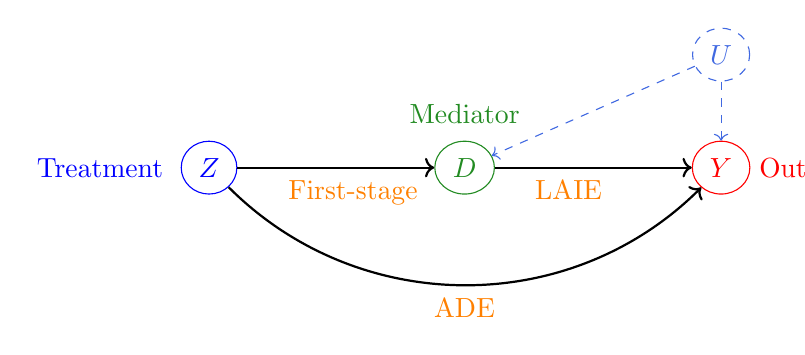
\begin{tikzpicture}
        \node[state,ForestGreen] (treatment) at (0,0) {$D$};
        \node[state,blue] (instrument) [left=2.5cm of treatment] {$Z$};
        \node[state,red] (outcome) [right=2.5cm of treatment] {$Y$};
        % Label Z, D, Y
        \node[color=ForestGreen] [above=0.1cm of treatment] (mediator) {Mediator};
        \node[color=blue] [left=0.1cm of instrument] {Treatment};
        \node[text width=0.1cm, color=red] [right=-0.01cm of outcome] {Outcome};
        % Draw the causal arrows
        \path[->, thick] (instrument) edge (treatment);
        \path[->, thick] (treatment) edge (outcome);
        \path[->, thick] (instrument) edge[bend right=45] (outcome);
        % Label direct and indirect effect
        \node[color=orange] [below left=-0.2cm and 0.2cm of treatment] {First-stage};
        \node[color=orange] [below right=-0.2cm and 0.5cm of treatment] {LAIE};
        \node[color=orange] [below=1.2cm of treatment] {ADE};
        % Add in the confounders
        %\node[state,RoyalPurple] (confounderX) [above=1.5cm of treatment] {$\vec{X}$};
        %\path[->,RoyalPurple] (confounderX) edge (treatment);
        %\node[color=RoyalPurple] [left=0.1cm of confounderX] {Observed controls};
        \node[state,dashed,RoyalBlue] (confounderU) [above=0.75cm of outcome] {$U$};
        \path[->,dashed,color=RoyalBlue] (confounderU) edge (treatment);
        \path[->,dashed,color=RoyalBlue] (confounderU) edge (outcome);
        %\node[color=RoyalBlue] [right=0.1cm of confounderU] {Unobserved confounder};
    \end{tikzpicture}
    \justify
    \footnotesize
    \textbf{Note}:
    This figures shows the structural causal model behind causal mediation.
    LAIE refers to the AIE (i.e., effect of the mediator $D \to Y$) local to $Z$ compliers, so that AIE $=$ average first-stage $\times$ LAIE.
    Unobserved confounder $U$ represents this paper's focus on the case that $D_i$ is not ignorable, by showing an implied unobserved confounder.
    \autoref{sec:regression} formally defines $U$ in this set-up.
\end{figure}

\subsection{Identifying Causal Mediation (CM) Effects}
The conventional approach to estimating direct and indirect effects assumes both $Z_i$ and $D_i$ are ignorable, conditional on a set of control variables $\vec X_i$.
\begin{definition}
    \label{dfn:seq-ign}
    Sequential Ignorability \citep{imai2010identification}.
    \begin{align}
        \label{eqn:seq-ign-Z}
        Z_i \indep  D_i(z), Y_i(z', d) \;\; &| \;\; \vec X_i,
            &\textnormal{ for } z, z', d = 0, 1 \\
        \label{eqn:seq-ign-D}
        D_i \indep Y_i(z', d) \;\; &| \;\; \vec X_i, Z_i = z', 
            &\textnormal{ for } z', d = 0, 1
    \end{align}
\end{definition}
Sequential ignorability assumes that the initial treatment $Z_i$ is assigned randomly, conditional on $\vec X_i$.
It then also assumes that, after $Z_i$ is assigned, that $D_i$ is assigned randomly conditional $\vec X_i, Z_i$.
If sequential ignorability, \ref{dfn:seq-ign}\eqref{eqn:seq-ign-Z} and \ref{dfn:seq-ign}\eqref{eqn:seq-ign-D}, holds then the ADE and AIE are identified by two-stage mean differences, after conditioning on $\vec X_i$.\footnote{
    \cite{imai2010identification} show a general identification statement; I show identification in terms of two-stage regression, notation for which is more familiar in economics.
    This reasoning is in line with G-computation reasoning \citep{robins1986g};
    \autoref{appendix:identification} states the \cite{imai2010identification} identification result, and then develops the two-stage regression notation which holds as a consequence of sequential ignorability.
}

\makebox[\textwidth]{\parbox{1.25\textwidth}{
\[ \E[D_i = d', \vec X_i]{
    \underbrace{\Egiven{Y_i}{Z_i = 1, D_i = d', \vec X_i} - \Egiven{Y_i}{Z_i = 0, D_i = d', \vec X_i}}_{\text{Second-stage regression, $Y_i$ on $Z_i$ holding $D_i$ constant}}}
    = \underbrace{\E{Y_i(1, D_i(Z_i)) - Y_i(0, D_i(Z_i))}}_{\text{Average Direct Effect (ADE)}} \]
\[ \E[Z_i = z', \vec X_i]{ \underbrace{\Big(
    \Egiven{D_i}{Z_i = 1, \vec X_i} - \Egiven{D_i}{Z_i = 0, \vec X_i} \Big)}_{\text{First-stage regression, $D_i$ on $Z_i$}}
    \times \underbrace{\Big(
    \Egiven{Y_i}{Z_i = z', D_i = 1, \vec X_i} - \Egiven{Y_i}{Z_i = z', D_i = 0, \vec X_i} \Big)}_{\text{Second-stage regression, $Y_i$ on $D_i$ holding $Z_i$ constant}} } \]
\[ = \underbrace{\E{Y_i(Z_i, D_i(1)) - Y_i(Z_i, D_i(0))}}_{\text{Average Indirect Effect (AIE)}} \]
}}
I refer to the estimands on the left-hand side as Causal Mediation (CM) estimands.
These estimands are typically estimated with linear models, with resulting estimates composed from OLS estimates \citep{imai2010identification}.
%\begin{align*}
%    D_i &= \phi + \pi Z_i
%        + \vec \psi_1' \vec X_i+ \eta_i \\
%    Y_i &= \alpha + \beta D_i + \gamma Z_i + \delta Z_i D_i
%        + \vec \psi_2' \vec X_i + \varepsilon_i
%\end{align*}
%And so the CM estimands are composed from OLS estimates,
%$\hat \gamma + \hat\delta \E{D_i}$ for the Average Direct Effect (ADE) and
%$\hat\pi \left(\hat \beta + \E{Z_i} \hat \delta \right)$ for the average indirect effect (AIE).
While this is the most common approach in the applied literature, I do not assume the linear model.
% of this problem as it assumes homogenous treatment effects and linear confounding.
Linearity assumptions are unnecessary to my analysis; it suffices to note that heterogeneous treatment effects and non-linear confounding would bias OLS estimates of CM estimands in the same manner that is well documented elsewhere (see e.g., \citealt{angrist1998estimating,sloczynski2022interpreting}).
This section focuses on problems that plague CM in practice, regardless of estimation method.
% As such, I focus my work on non-parametric identification, and employ semi- and non-parametric estimation methods in my empirical analysis  whenever possible to avoid these problems.

\subsection{Bias in Causal Mediation Estimates}
Applied research may use a natural experiment to justify the treatment $Z_i$ is ignorable, justifying assumption \ref{dfn:seq-ign}\eqref{eqn:seq-ign-Z}.
Rarely does research relying on a quasi-experimental research design employ an additional, overlapping identification design for $D_i$ to justify assumption \ref{dfn:seq-ign}\eqref{eqn:seq-ign-D} as part of the analysis.
One might consider using conventional CM methods to estimate direct and indirect effects, and learn about the mechanisms behind the treatment effect under study.This approach leads to biased estimates, and contaminates inference regarding direct and indirect effects.%\footnote{
    %    \cite{imai2013experimental} call attention to the need for a separate research design to isolate causal effects of $D_i$ in randomised controlled trials; \autoref{appendix:mediation-review} overviews literature, finding many papers that employ mediation methods with a research design for $Z_i$, but not for $D_i$.
    %}

\begin{theorem}
    \label{thm:selection-bias}
    Absent an identification strategy for the mediator, causal mediation estimates are at risk of selection bias.
    Suppose \ref{dfn:seq-ign}\eqref{eqn:seq-ign-Z} holds, but \ref{dfn:seq-ign}\eqref{eqn:seq-ign-D} does not.
    Then CM estimands are contaminated by selection bias and group differences.
\end{theorem}
\begin{proof}
    See \autoref{appendix:mediation-bias} for the extended proof.
\end{proof}
Below I present the relevant selection bias and group difference terms, omitting the conditional on $\vec X_i$ notation for brevity.

\noindent
For the direct effect: CM estimand $=$ ADE $+$ selection bias $+$ group differences.
\begin{align*}
    & \mathbb E_{D_i = d'} \Big[
        \Egiven{Y_i}{Z_i = 1, D_i = d'} - \Egiven{Y_i}{Z_i = 0, D_i = d'} \Big] \\
    & = \E{Y_i(1, D_i(Z_i)) - Y_i(0, D_i(Z_i))} \\
    & \;\;\;\; + \mathbb E_{D_i = d'} \Big[
        \Egiven{Y_i(0, D_i(Z_i))}{D_i(1) = d'} 
        - \Egiven{Y_i(0, D_i(Z_i))}{D_i(0) = d'} \Big] \\
    & \;\;\;\; + \E[D_i = d']{
        \Big(1 - \Prob{D_i(1) = d'} \Big)
        \left( \begin{aligned}
            &\Egiven{Y_i(1, D_i(Z_i)) - Y_i(0, D_i(Z_i))}{D_i(1) = d'} \\ 
            &  - \Egiven{Y_i(1, D_i(Z_i)) - Y_i(0, D_i(Z_i))}{D_i(0) = 1 - d'}
            \end{aligned} \right) }
\end{align*}

\noindent
For the indirect effect: CM estimand $=$ AIE $+$ selection bias $+$ group differences.\footnote{
    The bias terms here mirror those in \cite{heckman1998characterizing,angrist2009mostly} for a one dimensional $D\to Y$ treatment effect, when $D_i$ is not ignorable.
    \[ \Egiven{ Y_i}{D_i =1} - \Egiven{ Y_i}{D_i =0}
        %& = \text{ATT}
        %+ \Big( \Egiven{ Y_i(0)}{D_i =1} - \Egiven{ Y_i(0)}{D_i =0} \Big) \\
        = \text{ATE}
        + \underbrace{\Big( \Egiven{ Y_i(0)}{D_i =1} - \Egiven{ Y_i(0)}{D_i =0} \Big)}_{
            \text{Selection Bias}}
        + \underbrace{ \Prob{D_i=0} (\text{ATT}- \text{ATU}) }_{
            \text{Group-differences Bias}} \]
}
\begin{align*}
    &\E[Z_i = z']{
        \Big( \Egiven{D_i}{Z_i = 1} - \Egiven{D_i}{Z_i = 0} \Big) \times
        \Big( \Egiven{Y_i}{Z_i = z', D_i = 1} - \Egiven{Y_i}{Z_i = z', D_i = 0} \Big) } \\
    & = \E{Y_i(Z_i, D_i(1)) - Y_i(Z_i, D_i(0))} \\
    & \;\;\;\; + \Prob{D_i(1) = 1, D_i(0) = 0} \Big(
        \Egiven{Y_i(Z_i, 0)}{D_i = 1} - \Egiven{Y_i(Z_i, 0)}{D_i = 0} \Big) \\
    & \;\;\;\; + \Prob{D_i(1) = 1, D_i(0) = 0} \times \\
    & \;\;\;\; \;\; \left[ \begin{aligned}
        &\Big( 1 - \Prob{D_i=1} \Big)
        \left( \begin{aligned}
            &\Egiven{Y_i(Z_i, 1) - Y_i(Z_i, 0)}{D_i = 1} \\ 
            &  - \Egiven{Y_i(Z_i, 1) - Y_i(Z_i, 0)}{D_i = 0}
        \end{aligned} \right) \\
        &+ \left( \frac{1 - \Prob{D_i(1) = 1, D_i(0) = 0} }{
            \Prob{D_i(1) = 1, D_i(0) = 0}} \right)
        \left( \begin{aligned}
            &\Egiven{Y_i(Z_i, 1) - Y_i(Z_i, 0)}{D_i(1) = 0 \text{ or } D_i(0)=1} \\ 
            &  - \E{Y_i(Z_i, 1) - Y_i(Z_i, 0)}
        \end{aligned} \right)
    \end{aligned} \right]
\end{align*}

The selection bias terms come from systematic differences between groups who do and do not take the mediator ($D_i = 0$ versus $D_i = 1$), differences not fully unexplained by $\vec X_i$.
These selection bias terms would equal to zero if the mediator was ignorable \ref{dfn:seq-ign}\eqref{eqn:seq-ign-D}, but do not necessarily average to zero if not.
The group differences represent the fact that a matching estimator gives an average effect on the treated group and, when selection-on-observables does not hold, this is systematically different from the average effect \citep{heckman1998characterizing}.\footnote{
    The group differences term is longer for the AIE estimate, because the indirect effect is comprised from the effect of $D_i$ local to $Z_i$ compliers; a matching estimator gets the average effect on treated, and the longer term adjusts for differences with the complier average effect.
}$^{,}$\footnote{
    The selection-on-observables approach could, instead, focus on the average effect on treated populations (as do \citealt{keele2015identifying}).
    This runs into a problem of comparisons: CM estimates would give average effects on different treated groups.
    The CM estimand for the ADE on treated gives the ADE local to the $Z_i = 1$ treated group, and local to the $D_i = 1$ group for the AIE.
    In this way, these ADE and AIE on treated terms are not comparable to each other, so I focus on the true averages to avoid these misaligned comparisons.
}
The group differences term is a non-parametric framing of the bias from controlling for intermediate outcomes, previously studied only in a linear setting (i.e., bad controls in \citealt{cinelli2024crash}, or M-bias in \citealt{ding2015adjust}).

% Model-based Framework, mediation under Roy-style selection
\section{Causal Mediation in Applied Settings}
\label{sec:selection}
In this section, I further develop the issue of selection in causal mediation estimates. First, I show the non-parametric bias terms from above can be written as omitted variables bias in a regression framework.
Second, I show how selection bias operates in an applied model for selection into a mediator based on costs and benefits.

\subsection{Regression Framework}
\label{sec:regression}
Inference for direct and direct effects can be written in a regression framework, showing how correlation between the error term and the mediator persistently biases estimates.
Write $Y_i(Z, D)$ as a sum of observed factors $Z_i, \vec X_i$ and unobserved factors, $U_{1,i}, U_{0,i}$ (following the notation of \citealt{heckman2005structural}).
Put $\mu_D(Z; \vec X_i) = \Egiven{Y_i(Z_i, 0)}{\vec X}$, to give a representation of the average direct and indirect effects.
\begin{align*}
    \E{Y_i(Z_i, D_i(1)) - Y_i(Z_i, D_i(0))}
    &= \mathbb{E} \Big[ \Big( D_i(1) - D_i(0) \Big)
        \times \Big( \mu_1(Z_i; \vec X_i) - \mu_0(Z_i; \vec X_i) \Big) \Big], \\
    \E{Y_i(1, D_i(Z_i)) - Y_i(0, D_i(Z_i))}
        &= \mathbb{E} \Big[ \mu_{D_i}(1; \vec X_i) - \mu_{D_i}(0; \vec X_i) \Big].
\end{align*}
Then define the error terms.
\[ U_{0,i} = Y_i(Z_i, 0) - \mu_0(Z_i; \vec X_i),\;\;\;\;
U_{1,i} = Y_i(Z_i, 1) - \mu_1(Z_i; \vec X_i) \]
With this notation, observed data $Z_i, D_i, Y_i$ take the following representation, which characterises direct effects, indirect effects, and bias from selection.
\begin{align}
    \label{eqn:parametric-firststage}
    D_i &= \phi + \pi Z_i + \varphi(\vec X_i) + \eta_i  \\
    \label{eqn:parametric-secondstage}
    Y_i &= \alpha + \beta D_i + \gamma Z_i + \delta Z_i D_i
    + \zeta(\vec X_i)
    + \underbrace{U_{0,i} + D_i \left( U_{1,i} - U_{0,i} \right)}_{
        \text{Correlated error term.}}
\end{align}
First-stage \eqref{eqn:parametric-firststage} is identified, with $\phi, \varphi(\vec X_i)$ the intercept, and $\pi$ the average rate of compliance (which may depend on $\vec X_i$).
Second-stage \eqref{eqn:parametric-secondstage} is not identified without further assumptions.
$\alpha, \zeta(\vec X_i)$ are the intercept terms, and $\beta, \gamma, \delta$ are values that comprise mediation effects --- all whose values may depend on $\vec X_i$, see \autoref{appendix:regression-model} for full definitions.
$U_{0,i} + D_i \left( U_{1,i} - U_{0,i} \right)$ is the possibly correlated error term, which disrupts identification.
The average direct and indirect effects are averages of these coefficients.
\begin{align*}
    \E{Y_i(1, D_i(Z_i)) - Y_i(0, D_i(Z_i))}
        &= \E{\gamma + \delta D_i}, \\
    \E{Y_i(Z_i, D_i(1)) - Y_i(Z_i, D_i(0))}
        &= \E{\pi \left( \beta +  \delta Z_i \right)}.
\end{align*}
By construction, $U_i = U_{1, i} - U_{0, i}$ is an unobserved confounder.
The regression estimates of second-stage \eqref{eqn:parametric-secondstage} give unbiased estimates only if $D_i$ is also conditionally ignorable: $D_i \indep  U_i$.
If not, then regression estimates suffer from omitted variables bias if they do not adjust for the unobserved confounder $U_i$.

\subsection{Selection on Costs and Benefits}
The key to noting that CM is at risk of bias is noting that $D_i \indep  U_i$ is unlikely to hold in applied settings.
Without an identification strategy for $D_i$, in addition to one for $Z_i$, bias will persist, given how we conventionally think of selection into treatment.

Consider a model where individual $i$ selects into a mediator based on costs and benefits, after $Z_i, \vec X_i$ have been assigned.
Write $C_i$ for individual $i$'s costs of taking mediator $D_i$, and $\indicator{.}$ for the indicator function.
The Roy model has $i$ taking the mediator if the benefits exceed the costs.
\[ D_i \left( z' \right) = \indicator{
    \underbrace{Y_i\left( z', 1 \right) - Y_i\left( z', 0 \right)}_{\text{Benefits}}
    \geq \underbrace{C_i}_{\text{Costs}}}, \;\;\; \text{for } z'=0,1 \]
Paragraph here talking about why the Roy model is useful.
\citep{roy1951some,heckman1990empirical}.

Decompose the costs into its mean and unobserved error, as above $C_i(Z_i) = \mu_{C}(Z_i; \vec X_i) + U_{C,i}$, and collect the mean benefits, $\mu \coloneqq \mu_1 - \mu_0$.
So we can write the first-stage selection equation separated by observed means and unobserved errors.
\begin{align*}
    D_i(z') &= \indicator{
        \mu(z'; \vec X_i) - \mu_C(z'; \vec X_i) \geq U_{C,i} - U_i }
        , \;\;\; \text{for } z'=0,1
\end{align*}

Theorem: if selection is Roy style, and sequential ignorability holds, then unobserved benefits play no part in selection.
The only driver in differences in selection are differences in costs (and not benefits).
\[ \Egiven{ D_i(z') }{ U_i = u} = \Egiven{ D_i(z') }{ U_i = u'} \]
For all $u', u$ in the range of the distribution of $U_i$.
Proof: by contradiction, add to the appendix.
This could, for example, hold if $U_{1,i} - U_{0,i}$ is degenerate conditional on $\vec X_i$.

Short paragraph on why this means $\vec X_i$ must be incredibly rich.
Write about if $D_i$ is the choice to attend education, then $\vec X_i$ must soak up all gains to education.
Or assuming that all variation in $D_i$ comes from unobserved differences in take-up costs.
This is unlikely to hold true, absent a separate research design for $D_i$, limiting the selection to an information restricted version of the Roy model.

If not, then selection bias propagates, including writing here for what the selection bias term is equal to. 

% \subsection{Applied Settings}
% 
% Three parapgraphs on what goes on in empirical settings.
% Survey the papers, and speak about it heavily in one paragraph.
% 
% table:
% 
% name | $Z \to Y$ | design for $Z$ | Primary mediatory | controls | Possible $U$.
% 
% Discussion Section
\section{Solving Identification with a Control Function}
\label{sec:controlfun}
If your goal is to estimate CM effects, and you could control for unobserved selection terms $U_{0,i}, U_{1,i}$, then you would.
This ideal example would yield unbiased estimates.
% Alas, $U_i$ is by definition unobserved.
The control function method takes this insight seriously, providing conditions to model the implied unobserved confounding by $U_{0,i}, U_{1,i}$, and then control for it.\footnote{
    This section does not improve on the control function approach, instead only noting its utility to solve the identification problem of CM in a natural experiment setting.
}

Suppose the vector of control variables $\vec X_i$ has at least two entries;
denote $\vec X_i^{\text{IV}}$ as one entry in the vector, and $\vec X_i^-$ as the remaining rows.
\begin{definition}
    \label{dfn:controlfun-assumptions}
    Control function assumptions.
    \begin{align}
        \label{eqn:firststage-monotonicity}
        &\Probgiven{ D_i(1) \geq D_i(0) }{\vec X_i} = 1    \\
        \label{eqn:controlfun-iv}
        &\vec X_i^{\text{IV}} \text{ has the property }
        \partialdiff[\mu(\vec X_i)]{\vec X_i^{\text{IV}}} = 0 < \partialdiff[D_i(z')]{\vec X_i^{\text{IV}}}, \textnormal{ for } z' = 0, 1.
    \end{align}
\end{definition}
Assumption \ref{dfn:controlfun-assumptions}\eqref{eqn:firststage-monotonicity} is the (conditional) monotonicity assumption \citep{imbens1994identification}, which is untestable but acceptable in many empirical applications.
Assumption \ref{dfn:controlfun-assumptions}\eqref{eqn:controlfun-iv} is assuming that an instrument exists, which satisfies an exclusion restriction (i.e., not impacting mediator gains $\mu$), and has a non-zero influence on the mediator (i.e., strong first-stage).
The exclusion restriction is untestable, and must be guided by domain-specific knowledge; strength of the first-stage is testable, and must be justified with data by methods common in the instrumental variables literature.

Write $K_i$ for the expected values in predicting the mediator with observed data, as a function of the instrument $\vec X_i^{\text{IV}}$ and remaining controls $\vec X_i^-$.
Then take the two components of $K_i$ into $K_{0 ,i}, K_{1,i}$, corresponding to whether $i$ refuses or takes the mediator, respectively.
\begin{align*}
    K_i &= \Egiven{D_i}{Z_i, \vec X_i^{\text{IV}}, \vec X_i^-}, \\
    %K_i &= F_D \left( \bar D_i \mid Z_i, \vec X_i^{\text{IV}}, \vec X_i^- \right)
    K_{0,i} &= (1 - D_i) (1 - K_i), \;\;\;K_{1,i} = D_i K_i.
\end{align*}
Here, $K_i$ is equal to the conditional cumulative density function of $D_i$, $\Probgiven{D_i \leq d'}{Z_i, \vec X_i^{\text{IV}}, \vec X_i^-}$ for $d' = 0,1$.
Thus, $\left( K_{0 ,i}, K_{1,i}\right)$ serves as the control function in this setting.
\begin{theorem}
    \label{thm:controlfun}
    If \ref{dfn:controlfun-assumptions}\eqref{eqn:firststage-monotonicity} and \ref{dfn:controlfun-assumptions}\eqref{eqn:controlfun-iv} hold, then the mean potential differences
    (and thus CM effects)
    are identified by a control function approach.
    For each $z', d' = 0,1$
    \begin{align*}
        \Egiven{Y_i}{Z_i = 1, D_i = d', \vec X_i^-, K_{d',i}}
        - \Egiven{Y_i}{Z_i = 0, D_i = d', \vec X_i^-, K_{d',i}} 
        &= \Egiven{Y_i(1, d') - Y_i(0, d')}{\vec X_i^-} \\
        \Egiven{Y_i}{Z_i = z', D_i = 1, \vec X_i^-, K_{1,i}}
        - \Egiven{Y_i}{Z_i = z', D_i = 0, \vec X_i^-, K_{0,i}} 
        &= \Egiven{Y_i(z', 1) - Y_i(z', 0)}{\vec X_i^-}
    \end{align*}
    %\[ \Egiven{Y_i}{Z_i = z', D_i = d', \vec X_i^-, K_{d',i}}
    %    = \Egiven{Y_i(z', d')}{\vec X_i^-, K_{d',i}}
    %    , \;\; \text{ for } z', d' = 0,1. \]
\end{theorem}
\begin{proof}
    Special case of \citet[Theorem~1]{florens2008identification}, \citet[Theorem~3]{imbens2009identification}.
    %; see \autoref{appendix:controlfun-proof}.
\end{proof}

Assumption \ref{dfn:controlfun-assumptions}\eqref{eqn:firststage-monotonicity} guarantees that mediator $D_i(.)$ can be represented by a selection model \citep{vytlacil2002independence}, and \ref{dfn:controlfun-assumptions}\eqref{eqn:controlfun-iv} pins down a control function to identify the selection model.
The approach exploits the fact that the bias terms, coming from correlated the errors in \autoref{sec:regression}, can be estimated in a first-stage regression and included as controls in the second-stage.

If the underlying selection model had been a Roy model, the control function approach captures the unobserved benefits to taking mediator (independent of observed controls), and thus driving take-up of the mediator.
By incorporating the selection term derived from the first-stage model, the approach adjusts for the unobserved confounding from unobserved gains.
By contrast, assuming the mediator was ignorable would have been assuming that there are no unobserved benefits to the mediator take-up, so that there is no bias in the second-stage to account for.

The instrument is key to avoid distributional assumptions on the unobserved errors terms.
In the Roy model, the exclusion restriction can be satisfied in one key way: having an instrument for cost of mediator take up $\mu_C$.
If the instrument $\vec X_i^{\text{IV}}$ enters the cost function $\mu_C$, and not the benefits function $\mu$, then it satisfies the exclusion restriction.
In an applied world, $\vec X_i^{\text{IV}}$ can be data that explain cost differences in taking $D_i$, unrelated to other demographic information.
If a researcher is looking into higher education as a proposed mediator, then data which explains different costs of attending university (unrelated to education gains) can serve this role.
This is the logic behind the \cite{card1993using} distance-instrument, and can be extended to a CM setting with education as the mediator.

%\textbf{Senan note:} Needs a step involving re-weighting to the D(z) compliers in the LAIE estimation.
% This is done by estimating the second-stage with Abadie (2003) re-weighting.

\subsection{Estimation}
In practice, the approach relies on estimating the control function $K_i$, then including this in the second-stage as a control, and accounting for the estimation error for these in the standard errors.
These reliances come with major concerns.
First, it is imperative that the control function is estimated correctly, so it is necessary to employ a non-parametric approach to estimate the first-stage.
Second, the error terms enters the second-stage \eqref{eqn:parametric-secondstage} linearly, but is an unknown function (possibly non-linear) of the control function; thus, the second-stage must be estimated semi-parametrically.\footnote{
    In practice this can be done by adding a polynomial for the estimated control function into the outcome regression, or a splines approach, etc. 
}
Lastly, the standard errors must account for estimation uncertainty in the above two non-parametric steps.

These concerns are worth noting, because non-parametric regression is computationally demanding, and requires large samples for estimator convergence. 
Furthermore, these are estimated in two steps, so that the concerns are of greater importance.
Otherwise, small sample bias properties could even dominate the bias terms identified in \autoref{thm:selection-bias}.\footnote{
    See \cite[Section~6]{imbens2009identification} for a full discussion of the asymptotic theory of a control function estimator.
}
It is beyond the scope of this paper to develop the optimal procedure here, but these concerns are important.
% Senan note: future direction?  Needs consistency results, too.
% Needs a competent econometrician coauthor, as Senan is not....
For applied research aiming to estimate CM effects, the control function method is only appropriate in extremely large sample sizes, such as applications using administrative sources or biobanks.

With these concerns in mind, I propose the following method to estimate CM effects with a control function approach:
\begin{enumerate}
    \item Estimate the first-stage, $\Egiven{D_i}{Z_i, \vec X_i^{\text{IV}}, \vec X_i^-}$ with a non-parametric estimator (e.g., a probability forest, or fully interacted OLS specification).
    \item Calculate estimates of the control function:
    \begin{align*}
        \hat K_i &= \hat{\mathbb E} \left[D_i \middle\vert Z_i, \vec X_i^{\text{IV}}, \vec X_i^- \right], \\
        \hat K_{0,i} &= (1 - D_i) (1 - \hat K_i), \;\;\;
            \hat K_{1,i} = D_i \hat K_i.
    \end{align*}
    \item Estimate the second-stage with OLS (including an interaction term between $Z_i$ and $D_i$), and a semi-parametric regressor of the control function.
    \[ \mathbb{E} \left[Y_i \middle\vert Z_i, D_i, \vec X_i^-, \hat K_{0,i}, \hat K_{1,i}\right]
    = \beta D_i + \gamma Z_i + \delta Z_i D_i + l_0\left( \hat K_{0,i}\right) + l_1 \left( \hat K_{1,i} \right) \]
    $l_0(.), l_1(.)$ are semi-parametric nuisance functions, so can be approximated with a spline specification, for example.
    \item Calculate the ADE and AIE estimates from this second-stage.
    \begin{align*}
        \hat{\text{ADE}} &= \; \E{
            \hat{\mathbb{E}} \left[ Y_i \middle\vert Z_i = 1, D_i, \vec X_i^-, \hat K_i \right]
            - \hat{\mathbb{E}} \left[ Y_i \middle\vert Z_i = 0, D_i, \vec X_i^-, \hat K_i \right]} \\
        \hat{\text{AIE}} &= \; \mathbb E \left[ \begin{aligned} &\left(
            \hat{\mathbb{E}} \left[D_i \middle\vert Z_i = 1, \vec X_i^{\text{IV}}, \vec X_i^-\right]
            - \hat{\mathbb{E}} \left[D_i \middle\vert Z_i = 1, \vec X_i^{\text{IV}}, \vec X_i^-\right] \right) \\
            &\times \left(
                \hat{\mathbb{E}} \left[ Y_i \middle\vert Z_i, D_i = 1, \vec X_i^-, \hat K_i \right]
            - \hat{\mathbb{E}} \left[ Y_i \middle\vert Z_i, D_i = 0, \vec X_i^-, \hat K_i \right]
            \right) \end{aligned} \right]
    \end{align*}
    %\item Estimate the second-stage with weighted-least squares, including a control function with (estimated) $\kappa$-weights \citep{abadie2003semiparametric}.
    %\begin{align*}
    %    \hat\kappa_i &= \; 1 - \frac{(1 - Z_i)D_i}{
    %        1 - \hat\Pr\left(Z_i = 1 \middle\vert \vec X_i^-, \vec X_i^{\text{IV}}\right)} -
    %        \frac{Z_i (1 - D_i)}{
    %        \hat\Pr\left(Z_i = 1 \middle\vert \vec X_i^-, \vec X_i^{\text{IV}}\right)} \\
    %    \mathbb{E} \left[ \hat\kappa_i Y_i \middle\vert Z_i, D_i, \vec X_i^-, \hat K_i \right]
    %        &= \beta D_i + \gamma Z_i + \delta Z_i D_i + l\left( \hat K_i \right)
    %\end{align*}
    %Estimate the AIE from this second-stage.
    %\begin{align*}
    %    \hat{\text{AIE}} &= \; \mathbb E \left[ \begin{aligned} &\left(
    %        \hat{\mathbb{E}} \left[D_i \middle\vert Z_i = 1, \vec X_i^{\text{IV}}, \vec X_i^-\right]
    %        - \hat{\mathbb{E}} \left[D_i \middle\vert Z_i = 1, \vec X_i^{\text{IV}}, \vec X_i^-\right] \right) \\
    %        &\times \left(
    %            \hat{\mathbb{E}} \left[ \hat\kappa_i Y_i \middle\vert Z_i, D_i = 1, \vec X_i^-, \hat K_i \right]
    %        - \hat{\mathbb{E}} \left[ \hat\kappa_i Y_i \middle\vert Z_i, D_i = 0, \vec X_i^-, \hat K_i \right]
    %        \right) \end{aligned} \right]
    %    \end{align*}
    \item Bootstrap across the previous steps, to calculate standard errors for the respective ADE and AIE estimates.
\end{enumerate}

\subsection{Simulation Evidence}
The following simulation gives an example to show how this method works in practice.
Suppose data observed to the researcher $Z_i, D_i, Y_i, \vec X_i$ are drawn from the following data generating processes, for $i = 1, \hdots, N$.
\begin{align*}
    Z_i \sim \text{Binom}\left(0.5 \right),
    \;\; \vec X_i^- \sim N(4, 1),
    \;\; \vec X_i^{\text{IV}} \sim \text{Binom}\left( 0.5 \right), \\
    \left[ U_{0,i}, U_{1,i} \right]' \sim
    \text{BivariateNormal}\left( 0, 0, \sigma_0, \sigma_1, \rho \right),
    \;\; U_{C,i} \sim N(0, 0.25).
\end{align*}
$N = 10,000$ allows the large sample properties of the approach to operate; indeed, smaller sample sizes may not.

Suppose each $i$ chooses to take mediator $D_i$ by a Roy model, with following mean definitions for each $z', d' = 0, 1$.
\begin{align*}
    D_i(z') = \indicator{Y_i(z', 1) - Y_i(z', 0) \geq C_i},  \\
    \mu_{d'}\left(z' ; \vec X_i \right) = \vec X_i^- + \left( z' + d' + z' d' \right),
    \;\; \mu_{C}\left(z' ; \vec X_i \right) = 3z' + \vec X_i^- - \vec X_i^{\text{IV}}.
\end{align*}
Following \autoref{sec:selection}, these data have the following first and second-stage equations:
\begin{align*}
    D_i &= \indicator{-3Z_i - \vec X_i^{\text{IV}} + \vec X_i^- \geq U_{0,i} - U_{1,i}},  \\
    Y_i &= Z_i + D_i + Z_i D_i + \vec X_i^-
        + \left( 1 - D_i \right) U_{0,i} + D_i U_{1,i}.
\end{align*}
$Z_i$ has an effect on outcome $Y_i$, and it operates partially through mediator $D_i$.
$\mu_{D_i}(Z_i;.)$ has an interation term, $Z_i D_i$, so while each $Z_i$ and $D_i$ have a constant partial effect, the total effect depends on how many $i$ choose to take the mediator; in this simulation $\Prob{D_i = 1} = 0.437$, and $65.29\%$ of the sample are mediator compliers (where $D_i(1)=1$ and $D_i(0) = 0$).
This gives an average total effect ($Z\to Y$) value of 2.58, ADE 1.44, and AIE 1.13.\footnote{
    Note that average total effect $=$ ADE $+$ AIE, in this setting.
    $\Prob{Z_i=1} = 0.5$ ensures this equality, but is not guaranteed in general.
}

After $Z_i$ is assigned, $i$ chooses to take mediator $D_i$ by considering the costs and benefits --- which vary based on $Z_i$, demographic controls $\vec X_i$, and the (non-degenerate) unobserved error terms $U_{i,0}, U_{1,i}$.
As a result, sequential ignorability does not hold; the mediator is not conditionally ignorable.
Thus, a standard OLS (selection-on-observables) approach to CM does not give an estimate for how much of the $Z \to Y$ treatment effect goes through mediator $D$.
Instead, the OLS approach gives biased inference.

\begin{figure}[h!]
    \caption{Simulated Distribution of CM Effect Estimates.}
    \begin{subfigure}[c]{0.475\textwidth}
        \centering
        \caption{ADE.}
        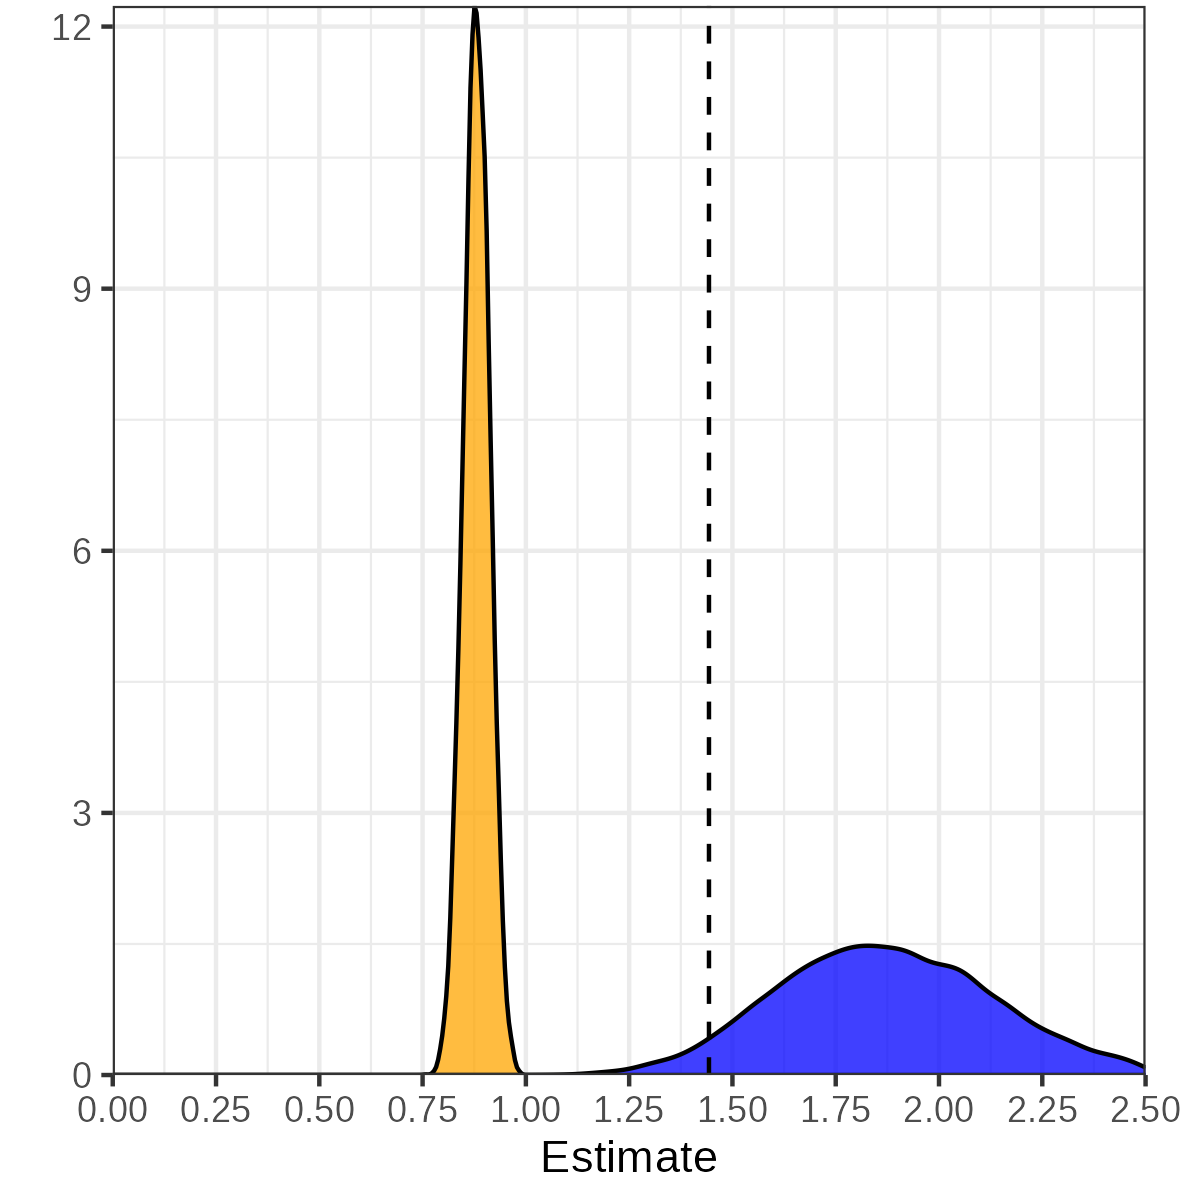
\includegraphics[width=\textwidth]{
            ../programs/simulations/sim-output/direct-boot.png}
    \end{subfigure}
    \begin{subfigure}[c]{0.475\textwidth}
        \centering
        \caption{AIE.}
        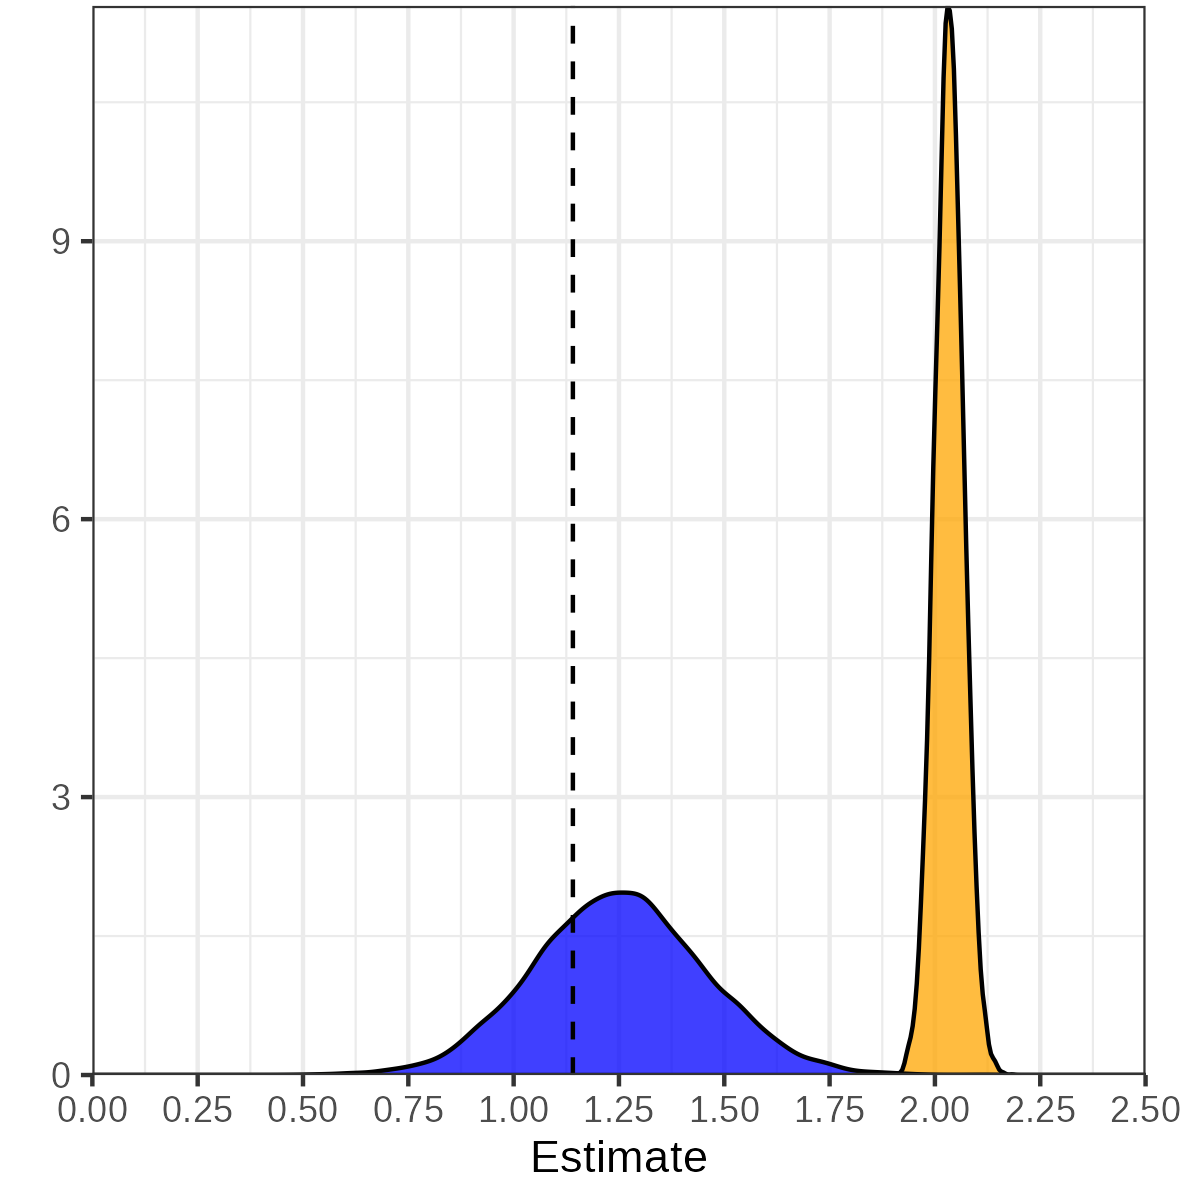
\includegraphics[width=\textwidth]{
            ../programs/simulations/sim-output/indirect-boot.png}
    \end{subfigure}
    \label{fig:cm-boot-dist}
    \justify
    \footnotesize    
    \textbf{Note:}
    These figures show the empirical density of point estimates, for 1,000 replications of the data generating process described above.
    The black dashed line is the true value;
    orange is the distribution of na\"ive OLS estimates, and blue the control function approach.
\end{figure}

The bias in OLS estimates comes from the unobserved error terms being related.
\autoref{fig:cm-boot-dist} shows the distribution of bootstrapped point estimates in this simulation, showing OLS against the control function approach.
The OLS approach implicitly assumes that the mediator is ignorable (when it is not), so its point estimates under and over-estimate the true ADE and AIE, respectively.
The distance between the OLS estimates and the true values are the underlying bias terms derived in \autoref{thm:selection-bias}.
In this data generating process, the OLS confidence interval do not overlap the true values for any standard level of significance.
The control function approach exhibits bias, though the 95\% confidence intervals cover the truth.

\begin{figure}[h!]
    \caption{Point Estimates of CM Effects, OLS versus Control Function.}
    \begin{subfigure}[c]{0.475\textwidth}
        \centering
        \caption{ADE.}
        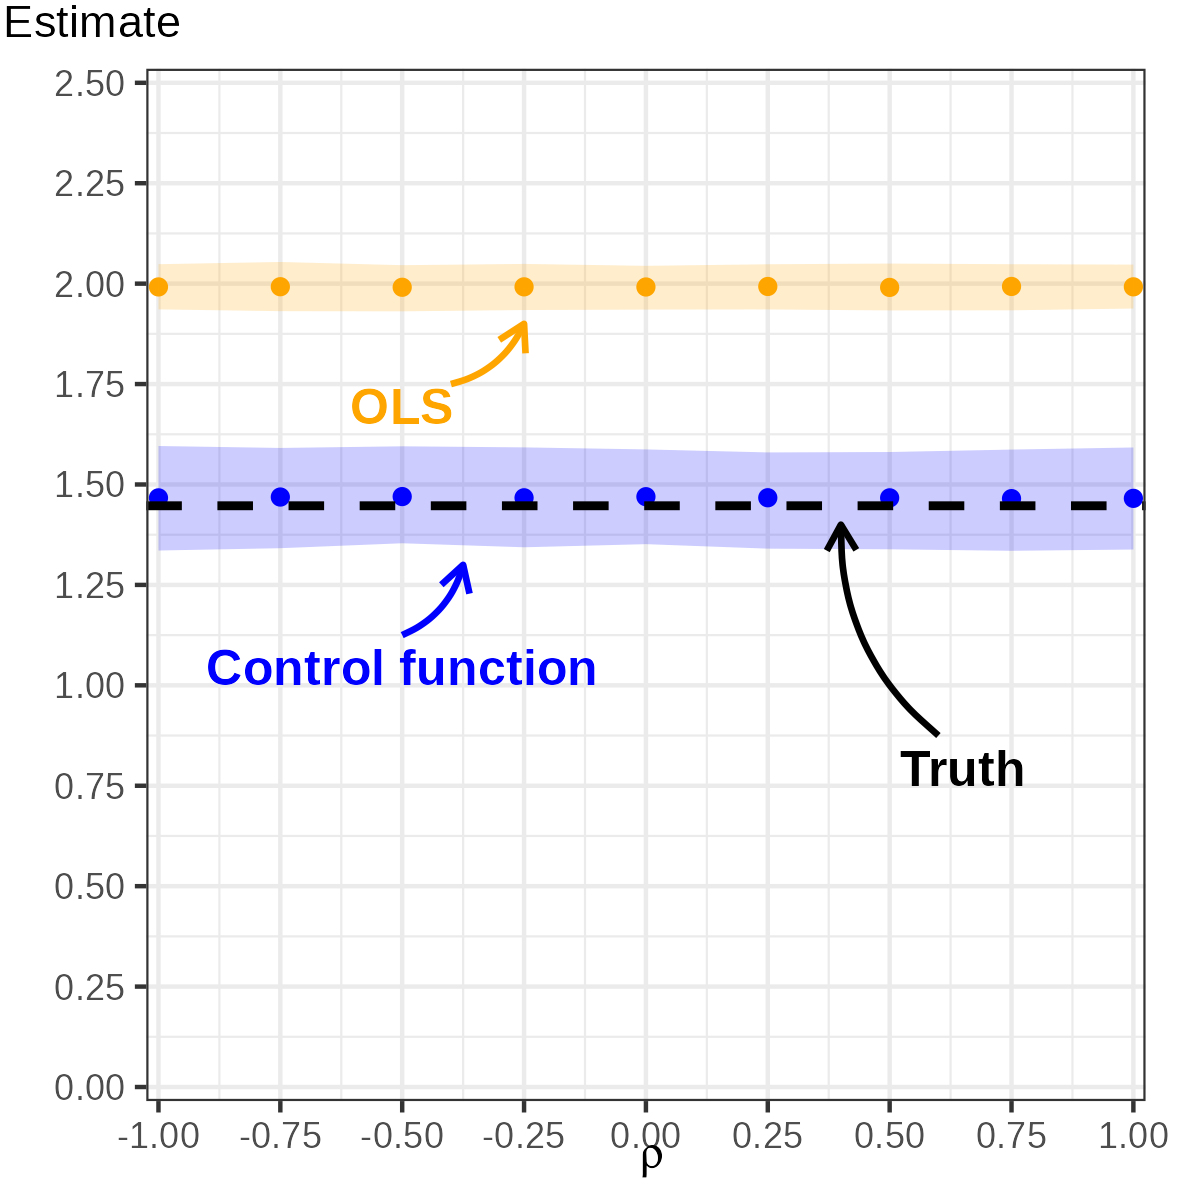
\includegraphics[width=\textwidth]{
            ../programs/simulations/sim-output/rho-directeffect-bias.png}
    \end{subfigure}
    \begin{subfigure}[c]{0.475\textwidth}
        \centering
        \caption{AIE.}
        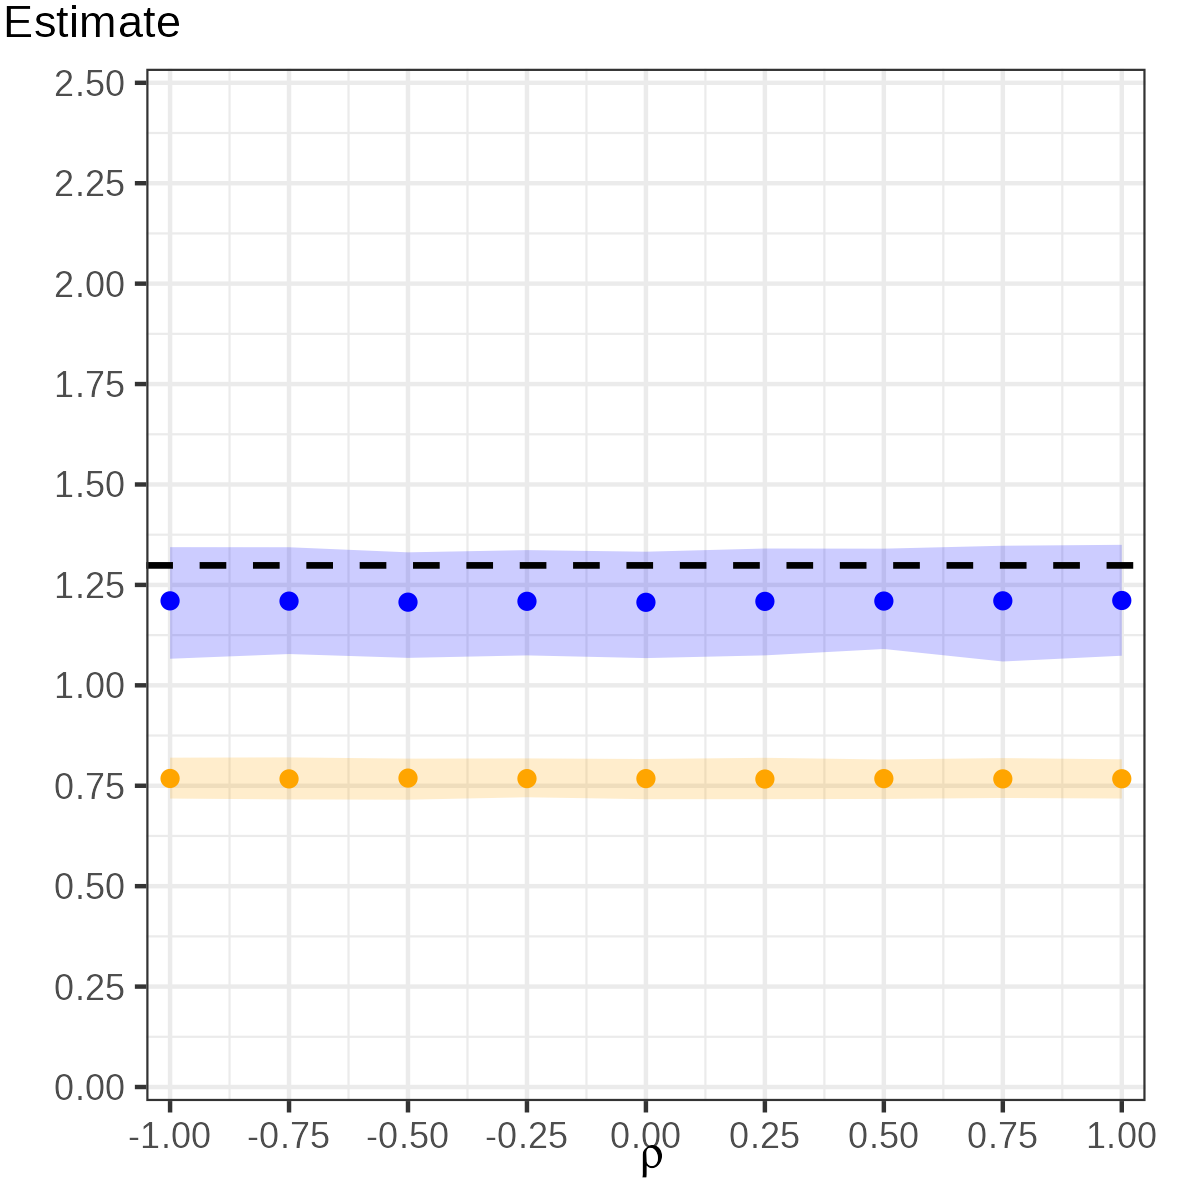
\includegraphics[width=\textwidth]{
            ../programs/simulations/sim-output/rho-indirecteffect-bias.png}
    \end{subfigure}
    \label{fig:rho-bias}
    \justify
    \footnotesize    
    \textbf{Note:}
    These figures show the OLS and control function point estimates of the ADE and AIE, for $N = 10,000$ sample size.
    The black dashed line is the true value, points are points estimates from data simulated with a given $\rho$ value and $\sigma_0 = 1, \sigma_1 = 2$, and shaded regions are the 95\% confidence intervals from 1,000 bootstraps each.
    Orange represents OLS estimates, blue the control function approach.
\end{figure}

The error terms determine the bias in OLS estimates of the ADE and AIE, so the bias varies for different values of the error-term parameters $\rho \in [-1, 1]$ and $\sigma_0, \sigma_1 \geq 0$.\footnote{
    Indeed, this setting has error terms following a bivariate normal distribution, so the canonical \cite{heckman1974shadow} selection model would produce the most efficient estimates by maximum likelihood.
    The control function approach avoids this assumption, and bias from breaking it, by relying on an instrument.
}
\autoref{fig:rho-bias} shows control function estimates against estimates calculated by standard OLS, showing 95\% confidence intervals calculated from 1,000 bootstraps.
The point estimates of the control function do not exactly equal the true values, as they are estimates from one simulation (not averages across many simulations as in \autoref{fig:cm-boot-dist}).
The control function approach improves on OLS estimates by correcting for the bias terms, with confidence regions overlapping the true values.\footnote{
    The code behind this simulation estimates the first-stage with an interacted OLS specification, and splines included for the continuous regressor $\vec X_i^-$.
    The second-stage is an OLS specification, including the (pre-estimated) control function with a spline specification.
}$^,$\footnote{
    In the appendix, \autoref{fig:sigma-bias} shows the same simulation while varying $\sigma_1$, with fixed $\sigma_0 = 1, \rho = 0.5$.
    The conclusion is the same as for varying the correlation coefficient, $\rho$, in \autoref{fig:rho-bias}.
}
This correction did not come for free: the standard errors are significantly greater in a control function approach than OLS.
Standard errors on the AIE are larger than those for the ADE, because the AIE estimates are first-stage times second-stage estimates (i.e., the same reasons instrumental variables estimates are less efficient than ideal OLS estimates). 
In this manner, this simulation shows the pros and cons of using the control function approach to estimating CM effects in practice.

% Conclusion Section
%%%%%%%%%%%%%%%%%%%%%%%%%%%%%%%%%%%%%%%%%
%% Conclusion section
\section{Summary and Concluding Remarks}
\label{sec:conclusion}

This paper studies the returns to higher education, using IV methods from the epidemiology literature and adjustments from the causal mediation literature to tackle violations of the exclusion restriction.
First, I derive identification of the average mechanism effect under a selection-on-observables type assumption, and partial identification when unobserved selection confounding.
I apply these methods to a sample of retirement age Americans in the years 1990--2021, using genetic information to instrument for higher education, estimating that higher education leads to roughly 40\% higher earnings (point estimates), or between 8--44\% higher earnings (partial bounds).
Additionally, women had significantly higher returns to higher education over this time period.

The methods here provide alternatives to assuming the exclusion restriction in empirical applications of IV models, so can be useful in sensitivity analyses for any application of IV methods.
Mendelian randomisation is a particularly useful application of IV methods, though the exclusion restriction is particularly problematic in practice.
The approach allows researchers to use MR to study effects of both health conditions and behaviours with significant selection-into-treatment concerns, such as higher education.

The approach could be used in AB tests, where a firm randomises a treatment and costs of a suspected mediator (if they do not want to also randomise a mediator fully).


% Bibliography
\singlespacing
\bibliographystyle{agsm}
\bibliography{sections/08-bibliography.bib}
%\bibliography{sections/08-bibliography-doi.bib}
% Appendix
\newpage
%%%%%%%%%%%%%%%%%%%%%%%%%%%%%%%%%%%%%%%%%
%% Appendix section
% Set-up the section.
%\newpage
\appendix
\setcounter{table}{0}
\renewcommand{\thetable}{A\arabic{table}}
\setcounter{figure}{0}
\renewcommand{\thefigure}{A\arabic{figure}}

% Start appendix
\section{Appendix}
\label{appendix}
This project used computational tools which are fully open-source.
%As such, all code and data involved in this project are available at this project's Github repository, available at \url{https://github.com/shoganhennessy/state-faculty-composition}.
%They may be used for replication, or as the basis for further work, as needed.
Any comments or suggestions may be sent to me at \href{mailto:seh325@cornell.edu}{\nolinkurl{seh325@cornell.edu}}, or raised as an issue on the Github project.

A number of statistical packages, for the R language \citep{R2023}, made the empirical analysis for this paper possible.
\begin{itemize}
    \item \textit{Tidyverse} \citep{tidyverse} collected tools for data analysis in the R language.
    \item \textit{DoubleML} \citep{DoubleML2020} implemented doubly robust methods used in the empirical analysis. 
    \item \textit{GRF} \citep{athey2019generalized,grf} compiled forest computational tools for the R language.
    \item \textit{Stargazer} \citep{stargazer} provided methods to efficiently convert empirical results into presentable output in \LaTeX.
\end{itemize}

\subsection{Identification in Causal Mediation}
\label{appendix:identification}
\citet[Theorem~1]{imai2010identification} states that the direct and indirect effects are identified under sequential ignorability, at each level of $Z_i = 0,1$.
For $z' = 0,1$: \\
\makebox[\textwidth]{\parbox{1.25\textwidth}{
\begin{align*}
    \E{ Y_i(1, D_i(z')) - Y_i(0, D_i(z'))}
    &= \int \int 
    \Big( \Egiven{ Y_i }{Z_i = 1, D_i, \vec X_i}
        - \Egiven{ Y_i }{Z_i = 0, D_i, \vec X_i} \Big)
            dF_{D_i \, | \, Z_i = z', \vec X_i} dF_{\vec X_i}, \\
    \E{ Y_i(z', D_i(1)) - Y_i(z', D_i(0))}
    &= \int \int \Egiven{ Y_i }{Z_i = z', D_i, \vec X_i}
    \Big( dF_{D_i \, | \, Z_i = 1, \vec X_i}
        - dF_{D_i \, | \, Z_i = 0, \vec X_i} \Big) dF_{\vec X_i}.
\end{align*}
}}
I focus on the averages, which are identified by consequence of the above.
\begin{align*}
    \E{ Y_i(1, D_i(Z_i)) - Y_i(0, D_i(Z_i))}
    &= \E[Z_i]{\Egiven{ Y_i(1, D_i(z')) - Y_i(0, D_i(z'))}{Z_i = z'}} \\
    \E{ Y_i(Z_i, D_i(1)) - Y_i(Z_i, D_i(0))}
    & = \E[Z_i]{\Egiven{ Y_i(z', D_i(1)) - Y_i(z', D_i(0))}{Z_i = z'}}
\end{align*}
My estimand for the average direct effect is a simple rearrangement of the above.
The estimand for the average indirect effect relies on a different sequence, relying on (1) sequential ignorability, (2) conditional monotonicity.
These give (1) identification of, and equivalence between, LADE conditional on $\vec X_i$ and ADE conditional on $\vec X_i$, (2) identification of the complier score.

\begin{align*}
    & \Egiven{ Y_i(Z_i, D_i(1)) - Y_i(Z_i, D_i(0))}{\vec X_i} \\
    & = \Probgiven{D_i(1) = 1, D_i(0) = 0}{\vec X_i}
        \Egiven{ Y_i(Z_i, 1) - Y_i(Z_i, 0)}{D_i(1) = 1, D_i(0) = 0, \vec X_i} \\
    & = \Probgiven{D_i(1) = 1, D_i(0) = 0}{\vec X_i}
        \Egiven{ Y_i(Z_i, 1) - Y_i(Z_i, 0)}{\vec X_i} \\
    & = \Big( \Egiven{D_i}{Z_i = 1, \vec X_i} - \Egiven{D_i}{Z_i = 0, \vec X_i}
        \Big) \; \Egiven{ Y_i(Z_i, 1) - Y_i(Z_i, 0)}{\vec X_i} \\
    & = \Big( \Egiven{D_i}{Z_i = 1, \vec X_i} - \Egiven{D_i}{Z_i = 0, \vec X_i}
        \Big)
        \Big( \Egiven{Y_i}{Z_i, D_i = 1, \vec X_i}
            - \Egiven{Y_i}{Z_i, D_i = 0, \vec X_i} \Big)
\end{align*}
Monotonicity is not technically required for the above.
Breaking monotonicity would not change the identification of any of the above; it would be the same except replacing the complier score with a complier or defier score, $\Probgiven{D_i(1) \neq D_i(0)}{\vec X_i} = \Egiven{D_i}{Z_i = 1, \vec X_i} - \Egiven{D_i}{Z_i = 0, \vec X_i}$.

\subsection{Continuous Average Causal Responses}
\label{appendix:continuous}
Section here relating the approach to the average causal response function (see e.g., Angrist Imbens JASA 1996, Andrew Bacon for DiD 2023).

\subsection{Previous Literature}
\label{appendix:mediation-review}

Create a table in this section that surveys previous research which employs mediation methods while having a clear causal design for $Z_i$, but not $D_i$.

\begin{tabular}{l l l l l}
    Paper & Field & Research Design for $Z_i$ & Research Design for $D_i$ & Selection bias? \\ \hline
    Paper name 1.    
\end{tabular}

\subsection{Bias in Mediation Estimates}
\label{appendix:mediation-bias}
Suppose that $Z_i$ is ignorable conditional on $\vec X_i$, but $D_i$ is not.

\subsubsection{Bias in Direct Effect Estimates}
To show that the conventional approach to mediation gives an estimate for the ADE with selection and non-complier bias, start with the components of the conventional estimands.
This proof starts with the relevant expectations, conditional on a specific value of $\vec X_i$.
For each $d' =0, 1$.
\begin{align*}
    \Egiven{Y_i}{Z_i = 1, D_i = d', \vec X_i}
    =& \Egiven{Y_i(1, D_i(Z_i))}{D_i(1) = d', \vec X_i}, \\
    \Egiven{Y_i}{Z_i = 0, D_i = d', \vec X_i}
    =& \Egiven{Y_i(0, D_i(Z_i))}{D_i(0) = d', \vec X_i}
\end{align*}
And so
\begin{align*}
    &  \Egiven{Y_i}{Z_i = 1, D_i = d', \vec X_i}
    - \Egiven{Y_i}{Z_i = 0, D_i = d', \vec X_i} \\
    =& \Egiven{Y_i(1, D_i(Z_i))}{D_i(1) = d', \vec X_i}
    - \Egiven{Y_i(0, D_i(Z_i))}{D_i(0) = d', \vec X_i} \\
    =& \Egiven{Y_i(1, D_i(Z_i)) - Y_i(0, D_i(Z_i))}{D_i(1) = d', \vec X_i} \\
    &+ \Egiven{Y_i(0, D_i(Z_i))}{D_i(1) = d', \vec X_i}
        - \Egiven{Y_i(0, D_i(Z_i))}{D_i(0) = d', \vec X_i} 
\end{align*}
The final term is a sum of the ADE, conditional on $D_i(1) = d'$, and a selection bias term --- difference in baseline terms between the (partially overlapping) groups for whom $D_i(1) = d'$ and $D_i(0) = d'$.

To reach the final term, note the following.
\begin{align*}
    &\Egiven{Y_i(1, D_i(Z_i)) - Y_i(0, D_i(Z_i))}{\vec X_i} \\    
    =& \Egiven{Y_i(1, D_i(Z_i)) - Y_i(0, D_i(Z_i))}{D_i(1) = d', \vec X_i} \\
    &+ \Big(1 - \Probgiven{D_i(1) = d'}{\vec X_i}\Big)
    \left( \begin{aligned}
        &\Egiven{Y_i(1, D_i(Z_i)) - Y_i(0, D_i(Z_i))}{D_i(1) = d', \vec X_i} \\ 
        & - \Egiven{Y_i(1, D_i(Z_i)) - Y_i(0, D_i(Z_i))}{D_i(1) = 1 - d', \vec X_i}
    \end{aligned} \right) 
\end{align*}
The second term is a difference term between the average and the average for relevant complier groups.

Collect everything together, as follows.
\begin{align*}
    &  \Egiven{Y_i}{Z_i = 1, D_i = d', \vec X_i}
    - \Egiven{Y_i}{Z_i = 0, D_i = d', \vec X_i} \\
    =& \underbrace{
        \Egiven{Y_i(1, D_i(Z_i)) - Y_i(0, D_i(Z_i))}{\vec X_i}}_{
            \text{ADE, conditional on }\vec X_i} \\
    &+ \underbrace{
        \Egiven{Y_i(0, D_i(Z_i))}{D_i(1) = d', \vec X_i}
            - \Egiven{Y_i(0, D_i(Z_i))}{D_i(0) = d', \vec X_i}}_{
                \text{Selection bias}} \\
    &+ \underbrace{\Big(1 - \Probgiven{D_i(1) = d'}{\vec X_i}\Big)
    \left( \begin{aligned}
        &\Egiven{Y_i(1, D_i(Z_i)) - Y_i(0, D_i(Z_i))}{D_i(1) = d', \vec X_i} \\ 
        & - \Egiven{Y_i(1, D_i(Z_i)) - Y_i(0, D_i(Z_i))}{D_i(1) = 1 - d', \vec X_i}
    \end{aligned} \right)}_{
        \text{Non-complier bias}}
\end{align*}
The proof is achieved by applying the expectation across $D_i = d'$, and $\vec X_i$.

\subsubsection{Bias in Indirect Effect Estimates}
To show that the conventional approach to mediation gives an estimate for the AIE with selection and non-complier bias, start with the definition of the ADE --- the direct effect among compliers times the size of the complier group.

This proof starts with the relevant expectations, conditional on a specific value of $\vec X_i$.
\begin{align*}
    &\Egiven{ Y_i(Z_i, D_i(1)) - Y_i(Z_i, D_i(0))}{\vec X_i} \\
    =& \Probgiven{D_i(1) = 1, D_i(0) = 0}{\vec X_i}
        \Egiven{ Y_i(Z_i, 1) - Y_i(Z_i, 0)}{D_i(1) = 1, D_i(0) = 0, \vec X_i}
\end{align*}
When $D_i$ is not ignorable, the bias comes from estimating the second term,\\ $\Egiven{ Y_i(Z_i, 1) - Y_i(Z_i, 0)}{D_i(1) = 1, D_i(0) = 0, \vec X_i}$.

For each $z' =0, 1$.
\begin{align*}
    \Egiven{Y_i}{Z_i = z', D_i = 1, \vec X_i}
    =& \Egiven{Y_i(z', 1)}{D_i = 1, \vec X_i}, \\
    \Egiven{Y_i}{Z_i = z', D_i = 0, \vec X_i}
    =& \Egiven{Y_i(z', 0)}{D_i = 0, \vec X_i}
\end{align*}
So compose the CM estimand, as follows.
\begin{align*}
    & \Egiven{Y_i}{Z_i = z', D_i = 1, \vec X_i}
    - \Egiven{Y_i}{Z_i = z', D_i = 0, \vec X_i} \\
    =& \Egiven{Y_i(z', 1)}{D_i = 1, \vec X_i}
        - \Egiven{Y_i(z', 0)}{D_i = 0, \vec X_i} \\
    =& \Egiven{Y_i(z', 1) - Y_i(z', 0)}{D_i = 1, \vec X_i}
    + \Egiven{Y_i(z', 0)}{D_i = 1, \vec X_i} - \Egiven{Y_i(z', 0)}{D_i = 0, \vec X_i}
\end{align*}
The final term is a sum of the AIE, among the treated group $D_i = 1$, and a selection bias term --- difference in baseline terms between the groups $D_i = 1$ and $D_i = 0$.

The AIE is the direct effect among compliers times the size of the complier group, so we need to compensate for the difference between the treated group $D_i = 1$ and complier group $D_i(1)= 1, D_i(0) = 0$.

Start with the difference between treated group's average and overall average.
\begin{align*}
    & \Egiven{Y_i(z', 1) - Y_i(z', 0)}{D_i = 1, \vec X_i} \\
    =& \Egiven{Y_i(z', 1) - Y_i(z', 0)}{\vec X_i} \\
    &+ \Big(1 - \Probgiven{D_i = 1}{\vec X_i} \Big)
    \left( \begin{aligned}
        &\Egiven{Y_i(z', 1) - Y_i(z', 0)}{D_i = 1, \vec X_i} \\ 
        &  - \Egiven{Y_i(z', 1) - Y_i(z', 0)}{D_i = 0, \vec X_i}
    \end{aligned} \right)
\end{align*}
Then the difference between the compliers' average and the overall average.
\begin{align*}
    & \Egiven{ Y_i(z', 1) - Y_i(z', 0)}{D_i(1) = 1, D_i(0) = 0, \vec X_i} \\
    =& \Egiven{Y_i(z', 1) - Y_i(z', 0)}{\vec X_i} \\
    & + \frac{1 - \Probgiven{D_i(1) = 1, D_i(0) = 0}{\vec X_i} }{
        \Probgiven{D_i(1) = 1, D_i(0) = 0}{\vec X_i}}
    \left( \begin{aligned}
        &\Egiven{Y_i(z', 1) - Y_i(z', 0)}{D_i(1) = 0 \text{ or } D_i(0)=1, \vec X_i} \\ 
        &  - \Egiven{Y_i(z', 1) - Y_i(z', 0)}{\vec X_i}
    \end{aligned} \right)
\end{align*}

Collect everything together, as follows.
\begin{align*}
    &  \Egiven{Y_i}{Z_i = z', D_i = 1, \vec X_i}
    - \Egiven{Y_i}{Z_i = z', D_i = 0, \vec X_i} \\
    =& \underbrace{
        \Egiven{Y_i(z', D_i(1)) - Y_i(z', D_i(0))}{\vec X_i}}_{
            \text{AIE, conditional on }\vec X_i, Z_i = z'} \\
    &+ \underbrace{
        \Egiven{Y_i(z', 0)}{D_i = 1, \vec X_i}
            - \Egiven{Y_i(z', 0)}{D_i = 0, \vec X_i}}_{
                \text{Selection bias}} \\
    &+ \underbrace{\left[ \begin{aligned}
        &\Big(1 - \Probgiven{D_i = 1}{\vec X_i} \Big)
        \left( \begin{aligned}
            &\Egiven{Y_i(z', 1) - Y_i(z', 0)}{D_i = 1, \vec X_i} \\ 
            &  - \Egiven{Y_i(z', 1) - Y_i(z', 0)}{D_i = 0, \vec X_i}
        \end{aligned} \right) \\
        &+ \frac{1 - \Probgiven{D_i(1) = 1, D_i(0) = 0}{\vec X_i} }{
            \Probgiven{D_i(1) = 1, D_i(0) = 0}{\vec X_i}} 
        \left( \begin{aligned}
            &\Egiven{Y_i(z', 1) - Y_i(z', 0)}{D_i(1) = 0 \text{ or } D_i(0)=1, \vec X_i} \\ 
            &  - \Egiven{Y_i(z', 1) - Y_i(z', 0)}{\vec X_i}
        \end{aligned} \right)
    \end{aligned} \right] }_{
        \text{Non-complier bias}}
\end{align*}
The proof is finally achieved by multiplying by the complier score, 
$\Probgiven{D_i(1) = 1, D_i(0) = 0}{\vec X_i}$
$= \Egiven{D_i}{Z_i = 1, \vec X_i} - \Egiven{D_i}{Z_i = 0, \vec X_i}$,
then applying the expectation across $Z_i = z'$, and $\vec X_i$.





\subsection{Proof of the Selection Model Representation}
\label{appendix:selection-model}
Write the proof in here, following \cite{vytlacil2002independence} construction in the forward direction.
Note that the notation needs updating for no exclusion restriction.

\subsection{A Regression Framework for Direct and Indirect Effects}
\label{appendix:regression-model}
Put $\mu_{D}(Z; \vec X) = \Egiven{Y_i(Z, D)}{\vec X}$ and $U_{D, i} = Y_i(Z,D) - \mu_D(Z; \vec X)$, so we have the following expressions.
\[ Y_i(Z_i, 0)
        = \mu_{0}(Z_i; \vec X_i) + U_{0,i}, \;\;
    Y_i(Z_i, 1)
        = \mu_{1}(Z_i; \vec X_i) + U_{1,i} \]

$U_{0,i}, U_{1,i}$ are error terms with unknown distributions, mean independent of $Z_i, \vec X_i$ by definition --- but possibly correlated with $D_i$.

$Z_i$ is independent of potential outcomes, so that $U_{0,i}, U_{1,i} \indep Z_i$.
Thus, the first-stage regression of $Z \to Y$ has unbiased estimates.
\begin{align*}
    D_i &= Z_i D_i(1) + (1 - Z_i) D_i(0) \\
        &= D_i(0) +
            Z_i \left[ D_i(1) - D_i(0) \right] \\
        &= \underbrace{\Egiven{D_i(0)}{\vec X_i}        
        }_{\text{Intercept}} +
            \underbrace{Z_i \E{ D_i(1) - D_i(0)}}_{
                \text{Regressor}} \\
            & \;\;\;\; + \underbrace{
                D_i(0) - \Egiven{D_i(0)}{\vec X_i}
                + Z_i \big( D_i(1) - D_i(0) - \Egiven{ D_i(1) - D_i(0)}{\vec X_i}\big)}_{
                \text{Mean-zero independent error term, since }Z_i \indep D_i \; | \; \vec X_i} \\
        &\eqqcolon \phi + \pi Z_i + \varphi(\vec X_i) + \eta_i \\
    \implies \Egiven{D_i}{Z_i, \vec X_i}&=
        \phi + \pi Z_i + \varphi(\vec X_i)
        \text{, and thus unbiased estimates since } Z_i \indep \phi, \eta_i.
\end{align*}

$Z_i$ is also assumed independent of potential outcomes $Y_i(,.,)$, so that $U_{0,i}, U_{1,i} \indep Z_i$.
Thus, the reduced form regression $Z \to Y$ also leads to unbiased estimates.

The same cannot be said of the regression that estimates direct and indirect effects, without further assumptions.
\begin{align*}
    Y_i &= Z_i Y_i(1, D_i(1)) + (1 - Z_i) Y_i(0, D_i(0)) \\
        &= Z_i D_i Y_i(1, 1) \\
        & \;\;\;\; + (1 - Z_i) D_i Y_i(0, 1) \\
        & \;\;\;\; + Z_i (1 - D_i) Y_i(1, 0) \\
        & \;\;\;\; + (1 - Z_i) (1 - D_i) Y_i(0, 0) \\
        &= Y_i(0, 0) \\
        & \;\;\;\; + Z_i \left[Y_i(1, 0) - Y_i(0, 0) \right] \\
        & \;\;\;\; + D_i \left[Y_i(0, 1) - Y_i(0, 0) \right] \\
        & \;\;\;\; + Z_i D_i \left[Y_i(1, 1) - Y_i(1, 0)
            - \left( Y_i(0, 1) - Y_i(0, 0) \right)\right]
\end{align*}
And so $Y_i$ can be written as a regression equation in terms of the observed factors and error terms.
\begin{align*}
    Y_i &= \mu_0(0; \vec X_i) \\
        & \;\;\;\; + D_i \left[\mu_1(0; \vec X_i) - \mu_0(0; \vec X_i) \right] \\
        & \;\;\;\; + Z_i \left[\mu_0(1; \vec X_i) - \mu_0(0; \vec X_i) \right] \\
        & \;\;\;\; + Z_i D_i \left[\mu_1(1; \vec X_i) - \mu_0(1; \vec X_i)
            - \left( \mu_1(0; \vec X_i) - \mu_0(0; \vec X_i) \right)\right] \\
        & \;\;\;\; + U_{0,i} + D_i \left( U_{1,i} - U_{0,i} \right) \\
        &\eqqcolon
            \alpha + \beta D_i + \gamma Z_i + \delta Z_i D_i
            + \zeta(\vec X_i)
            + U_{0,i} + D_i \left( U_{1,i} - U_{0,i} \right)
\end{align*}
With the following definitions:
\begin{itemize}
    \item $\alpha = \E{\mu_0(0; \vec X_i)}$ and $\zeta(\vec X_i) = \mu_0(0; \vec X_i) - \alpha$ are the intercept terms.
    \item $\beta = \mu_1(0; \vec X_i) - \mu_0(0; \vec X_i)$ is the indirect effect under $Z_i = 0$
    \item $\gamma = \mu_0(1; \vec X_i) - \mu_0(0; \vec X_i)$ is the direct effect under $D_i = 0$.
    \item $\gamma = \mu_1(1; \vec X_i) - \mu_0(1; \vec X_i)- \left( \mu_1(0; \vec X_i) - \mu_0(0; \vec X_i) \right)$ is the interaction effect.
    \item $U_{0,i} + D_i \left( U_{1,i} - U_{0,i} \right)$ is the remaining error term.
\end{itemize}
This sequence gives us the resulting regression equation:
\[ \Egiven{Y_i}{Z_i, D_i, \vec X_i} =
    \alpha
    + \beta D_i
    + \gamma Z_i
    + \delta Z_i D_i
    + \zeta(\vec X_i)
    + \Egiven{D_i \left( U_{1,i} - U_{0,i} \right)}{\vec X_i} \]
Taking the conditional expectation, and collecting for the expressions of the direct and indirect effects:\footnote{
    These equations have simpler expressions after assuming constant treatment effects in a linear framework;
    I have avoided this as having compliers, and controlling for observed factors $\vec X_i$ only makes sense in the case of heterogeneous treatment effects.
}
\begin{align*}
    \E{Y_i(Z_i, D_i(1)) - Y_i(Z_i, D_i(0))}
        &= \E{\pi \left( \beta +  Z_i \delta \right)} \\
    \E{Y_i(1, D_i(Z_i)) - Y_i(0, D_i(Z_i))}
        &= \E{\gamma + \delta D_i}
\end{align*}
These terms are conventionally estimated in a simultaneous regression \citep{imai2010identification}.

If sequential ignorability does not hold, then the regression estimates from estimating the mediation equations (without adjusting for the contaminated bias term) suffer from omitted variables bias.

\begin{align*}
    \E[\vec X_i]{\Egiven{Y_i}{Z_i = D_i = 0, \vec X_i}}
        &= \E\alpha + \E{D_i \left( U_{1,i} - U_{0,i} \right)} \\
    \E[\vec X_i]{\Egiven{Y_i}{Z_i = 0, D_i = 1, \vec X_i}
        - \Egiven{Y_i}{Z_i = 0, D_i = 0, \vec X_i}}
        &= \E\beta + \frac{
        \Cov{D_i,\; D_i \left( U_{1,i} - U_{0,i} \right)}}{\Var{D_i}} \\
    \E[\vec X_i]{\Egiven{Y_i}{Z_i = 1, D_i = 0, \vec X_i}
        - \Egiven{Y_i}{Z_i = 0, D_i = 0, \vec X_i}}
        &= \E\gamma + \frac{
        \Cov{Z_i,\; D_i \left( U_{1,i} - U_{0,i} \right)}}{\Var{Z_i}} \\
    \E[\vec X_i]{\begin{aligned}
        &\Egiven{Y_i}{Z_i = 1, D_i = 1, \vec X_i}
            - \Egiven{Y_i}{Z_i = 1, D_i = 0, \vec X_i} \\
            &- \left( \Egiven{Y_i}{Z_i = 0, D_i = 1, \vec X_i}
                - \Egiven{Y_i}{Z_i = 0, D_i = 0, \vec X_i} \right)
        \end{aligned}}
    &= \E\delta + \frac{
        \Cov{Z_i D_i,\; D_i \left( U_{1,i} - U_{0,i} \right)}}{\Var{Z_i D_i}}
\end{align*}
And so the direct and indirect effect estimates are contaminated by these bias terms.

% Senan note: should write CM estimand = \E{\gamma + \delta D_i} + bias, where bias is some Cov term.

\end{document}
